\section{Pianificazione}

	Per gestire lo sviluppo del progetto e soddisfare le scadenze riportate nella sottosezione \hyperref[riferimento_scadenze]{\S1.5}, il gruppo ha deciso di suddividere il periodo che va dalla sua formazione fino al completamento del progetto nelle seguenti fasi:
	\begin{itemize}
		\item analisi dei requisiti;
		\item consolidamento dei requisiti;
		\item progettazione della Technology Baseline;
		\item 12 incrementi;
		\item validazione e collaudo.
	\end{itemize}
	Ogni fase è suddivisa in più periodi, ognuno dei quali individua più attività, al suo interno, le quali possono essere svolte sia sequenzialmente, sia con un certo grado di parallelismo, in base alle dipendenze che sussistono tra di loro.
	
	\subsection{Analisi dei requisiti}
	
		La fase di analisi dei requisiti ha inizio il giorno 2019-11-15, successivamente alla formazione dei gruppi, ed è suddivisa in quattro periodi, con termine fissato per il giorno 2020-01-14, data della consegna dei documenti in ingresso alla revisione dei requisiti del 2020-01-21.
		
		\subsubsection{Ruoli attivi}
		
			Durante questa fase è necessaria la presenza dei seguenti ruoli:
			\begin{itemize}
				\item responsabile;
				\item amministratore;
				\item analista;
				\item verificatore.
			\end{itemize}
		
		\subsubsection{Periodi e attività}
		
			La fase di analisi dei requisiti è stata suddivisa nei seguenti quattro periodi:
			
			\paragraph{Primo periodo (dal 2019-11-15 al 2019-12-06)}
			
				\begin{itemize}
					\item \textbf{analisi dei capitolati:} studio individuale dei capitolati e discussione interna al gruppo dei pro e contro individuati da ogni componente, in modo da indirizzare l'interesse del gruppo su certi capitolati piuttosto che su altri;
					\item \textbf{ricerca:} individuazione e studio degli strumenti e delle tecnologie di supporto da utilizzare per la gestione del progetto;
					\item \textbf{normazione:} scelta delle regole da adottare durante lo sviluppo del progetto riguardanti la documentazione, la verifica e la gestione della configurazione;
					\item \textbf{pianificazione delle attività:} decisione dell'organizzazione interna al gruppo riguardo i ruoli da assegnare ed i compiti da svolgere;
					\item \textbf{studio di fattibilità:} impostato sulla base dell'analisi dei capitolati fatta in precedenza;
					\item \textbf{analisi di qualità:} analisi preliminare riguardante le metriche da utilizzare per controllare e garantire la qualità del prodotto;
					\item \textbf{verifica:} controllo della qualità di tutti i prodotti sviluppati durante il periodo attuale.
				\end{itemize}
			
			\paragraph{Secondo periodo (dal 2019-12-07 al 2019-12-16)}
			
				\begin{itemize}
					\item \textbf{scelta del capitolato:} decisione definitiva riguardo il capitolato scelto;
					\item \textbf{studio di fattibilità:} fine dello studio di fattibilità, basato al capitolato scelto;
					\item \textbf{normazione:} scelta delle regole da adottare durante lo sviluppo del progetto riguardanti i processi primari e processi organizzativi;
					\item \textbf{analisi di qualità:} analisi preliminare riguardante le metriche da utilizzare per controllare e garantire la qualità del prodotto;
					\item \textbf{ricerca:} individuazione e studio degli strumenti e delle tecnologie implicate dal capitolato scelto, da utilizzare durante lo svolgimento del progetto;
					\item \textbf{verifica:} controllo della qualità di tutti i prodotti sviluppati durante il periodo attuale.
				\end{itemize}
			
			\paragraph{Terzo periodo (dal 2019-12-17 al 2019-12-31)}
			
				\begin{itemize}
					\item \textbf{normazione:} scelta delle regole da adottare durante lo sviluppo del progetto riguardanti i processi di supporto non ancora discussi;
					\item \textbf{analisi dei casi d'uso:} analisi del prodotto e dei casi d'uso;
					\item \textbf{pianificazione:} organizzazione interna al gruppo riguardo la pianificazione dell'intero progetto;
					\item \textbf{analisi dei rischi:} individuazione dei rischi che possono presentarsi nello svolgimento del progetto;
					\item \textbf{ricerca:} studio autonomo degli strumenti e le tecnologie da utilizzare per lo sviluppo del progetto;
					\item \textbf{verifica:} controllo della qualità di tutti i prodotti sviluppati durante il periodo attuale.
				\end{itemize}
			
			\paragraph{Quarto periodo (dal 2020-01-01 al 2020-01-14)}
			
				\begin{itemize}
					\item \textbf{analisi dei requisiti:} analisi dei requisiti e tracciamento;
					\item \textbf{stesura della lettera di presentazione:} scrittura della lettera di presentazione con la quale ci si candida alla revisione dei requisiti;
					\item \textbf{aggiornamento della pianificazione};
					\item \textbf{aggiornamento della qualità};
					\item \textbf{ricerca:} studio autonomo degli strumenti e le tecnologie da utilizzare per lo sviluppo del progetto;
					\item \textbf{verifica:} controllo della qualità di tutti i prodotti sviluppati durante il periodo attuale.
				\end{itemize}
        
        \begin{landscape}

          \begin{figure}[H]
            \centering
            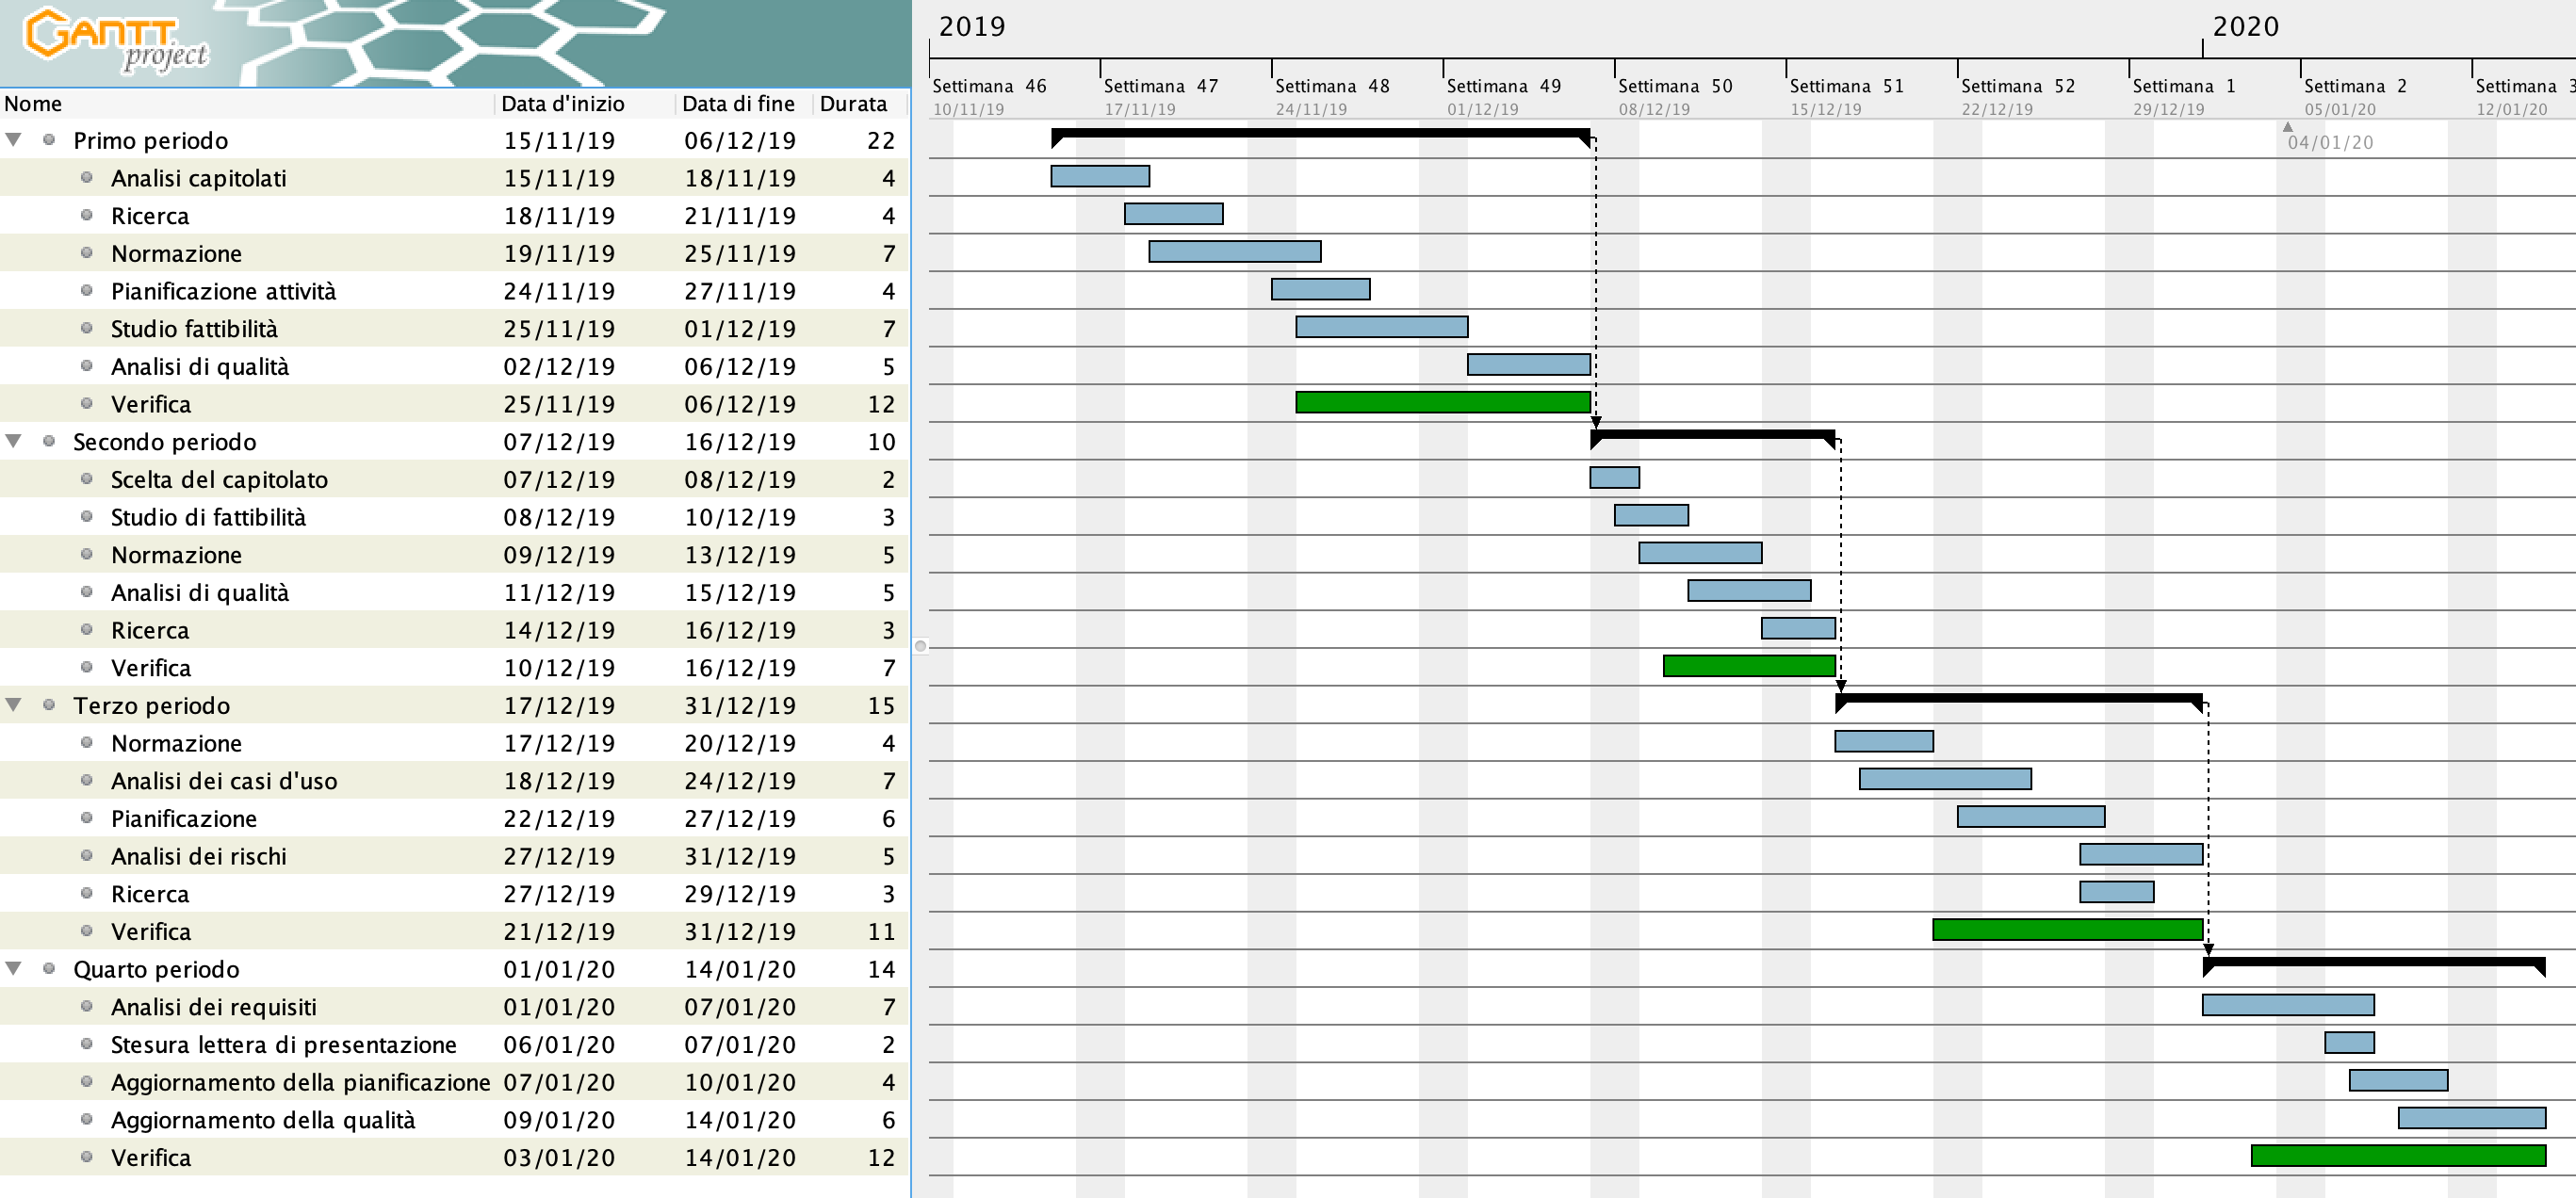
\includegraphics[width=\linewidth]{images/ganttAnalisi}
            \caption{Diagramma di Gantt della fase di analisi dei requisiti}
          \end{figure}

		\end{landscape}
		
		\subsection{Consolidamento dei requisiti}
		
			L'attività di consolidamento dei requisiti ha inizio il giorno 2020-01-15, successivamente alla consegna del materiale in ingresso alla revisione dei requisiti, ed è suddivisa in due periodi, con termine fissato per il giorno 2020-01-20, che precede la revisione dei requisiti del 2020-01-21.
			
			\subsubsection{Ruoli attivi}
			
				Durante questa fase è necessaria la presenza dei seguenti ruoli:
				\begin{itemize}
					\item responsabile;
					\item amministratore;
					\item analista.
				\end{itemize}
			
			\subsubsection{Periodi e attività}
			
				La fase di consolidamento dei requisiti è stata suddivisa nei seguenti due periodi:
				
				\paragraph{Primo periodo (dal 2020-01-15 al 2020-01-17)}
				
					\begin{itemize}
						\item \textbf{preparazione presentazione:} redazione della presentazione da portare in sede di revisione e studio individuale.
					\end{itemize}
				
				\paragraph{Secondo periodo (dal 2020-01-18 al 2020-01-21)}
				
					\begin{itemize}
						\item \textbf{analisi dei requisiti:} revisione ed eventuale aggiornamento dei requisiti.
					\end{itemize}

		\begin{landscape}

          \begin{figure}[H]
            \centering
            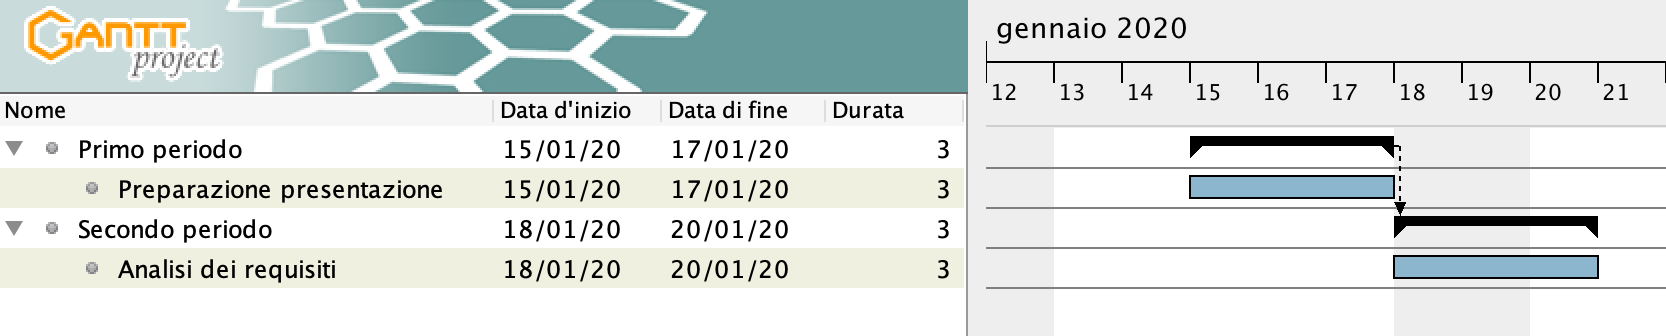
\includegraphics[width=\linewidth]{images/ganttConsolidamento}
            \caption{Diagramma di Gantt per la fase di consolidamento dei requisiti}
          \end{figure}		

		\end{landscape}

		\subsection{Progettazione della technology baseline}
	
			La fase di progettazione della technology baseline ha inizio il giorno 2020-01-22, successivamente alla revisione dei requisiti, ed è composta di un unico periodo, con termine fissato per il giorno 2020-03-15, che precede la revisione di progettazione del 2020-03-16.
			
			\subsubsection{Ruoli attivi}
			
				Durante questa fase è necessaria la presenza dei seguenti ruoli:
				\begin{itemize}
					\item responsabile;
					\item amministratore;
					\item analista;
					\item progettista;
					\item verificatore.
				\end{itemize}
			
			\subsubsection{Periodi e attività}
			
				La fase di progettazione della technology baseline è stata suddivisa in un solo periodo sufficientemente lungo per svolgere tutte le attività previste.
				
				\paragraph{Unico periodo (dal 2020-01-22 al 2020-02-04)}
				
					\begin{itemize}
					 	\item \textbf{normazione:} revisione ed eventuale aggiornamento delle norme;
					 	\item \textbf{aggiornamento della pianificazione};
					 	\item \textbf{aggiornamento della qualità};
					 	\item \textbf{analisi dei requisiti:} revisione ed eventuale aggiornamento dei casi d'uso e dei requisiti, in base alle indicazioni ricevute;
					 	\item \textbf{ricerca:} studio autonomo degli strumenti e le tecnologie da utilizzare per lo sviluppo del progetto;
					 	\item \textbf{progettazione:} progettazione dell'architettura del sistema e di un primo \glock{proof of concept};
					 	\item \textbf{verifica:} controllo della qualità di tutti i prodotti sviluppati durante il periodo attuale;
					 	\item \textbf{stesura della lettera di presentazione:} scrittura della lettera di presentazione con la quale ci si candida alla revisione di progettazione.
					\end{itemize} 	
		
        \begin{landscape}

          \begin{figure}[H]
            \centering
            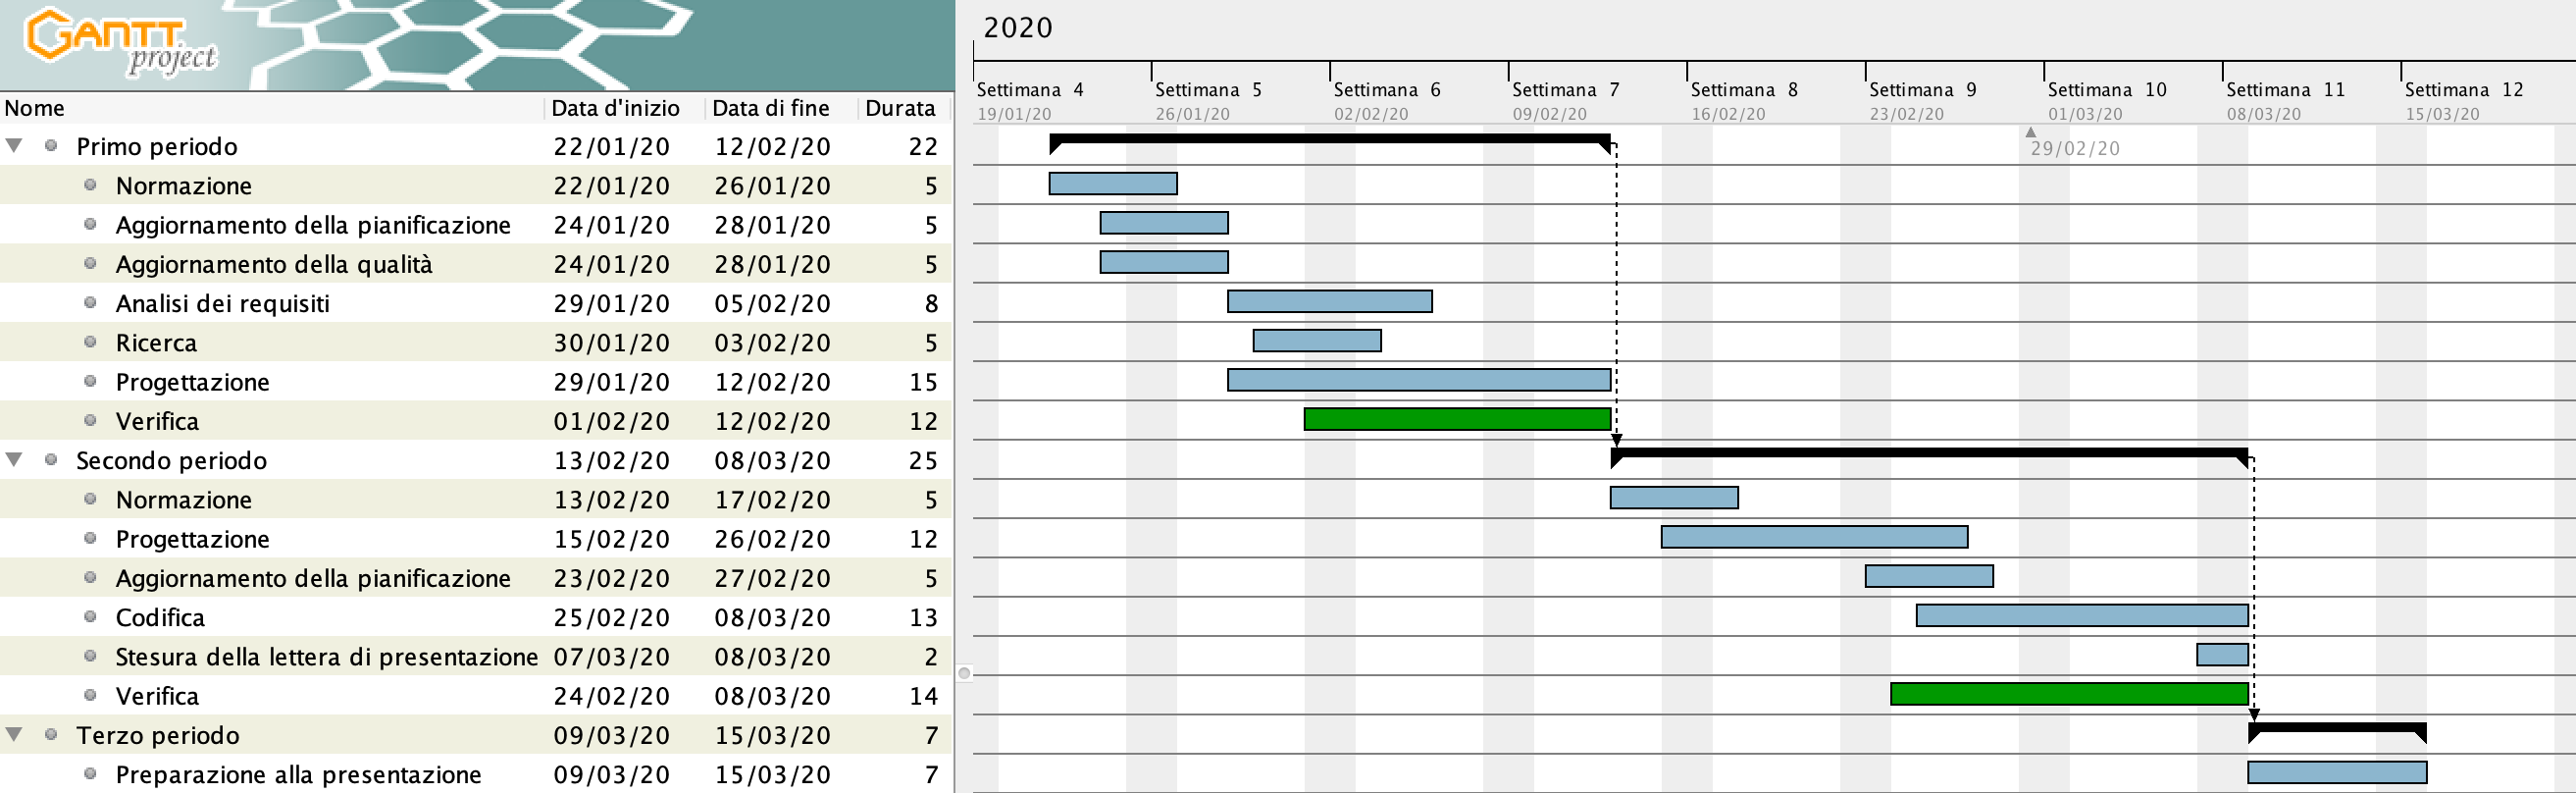
\includegraphics[width=\linewidth]{images/ganttTechBase} %TOUPDATE
            \caption{Diagramma di Gantt della fase di progettazione della technology baseline}
          \end{figure}

		\end{landscape}		


		% ============================================

		\subsection{Incremento I}
			
			L'incremento I prevede la progettazione di dettaglio e codifica delle componenti software per andare a costituire un \glock{proof of concept}. Si prevede di svolgere quanto segue:
			\begin{itemize}
				\item configurazione di \glock{Apache Kafka}.
			\end{itemize}
			
			\subsubsection{Ruoli attivi}
			
				Durante questa fase è necessaria la presenza dei seguenti ruoli:
				\begin{itemize}
					\item responsabile;
					\item amministratore;
					\item analista;
					\item progettista;
					\item programmatore;
					\item verificatore.
				\end{itemize}
			
			\subsubsection{Periodi e attività}
			
				L'incremento viene svolto in un unico periodo di breve durata.
				
				\paragraph{Unico periodo (dal 2020-02-05 al 2020-02-09)}
				
					\begin{itemize}
						\item \textbf{analisi delle tecnologie:} analisi del funzionamento di \glock{Apache Kafka} e di \glock{Docker};
						\item \textbf{progettazione:} progettazione della configurazione per \glock{Apache Kafka} e integrazione con \glock{Docker};
						\item \textbf{codifica:} implementazione della configurazione;
						\item \textbf{verifica:} controllo sul funzionamento della configurazione.
					\end{itemize} 			

		\begin{landscape}

          \begin{figure}[H]
            \centering
            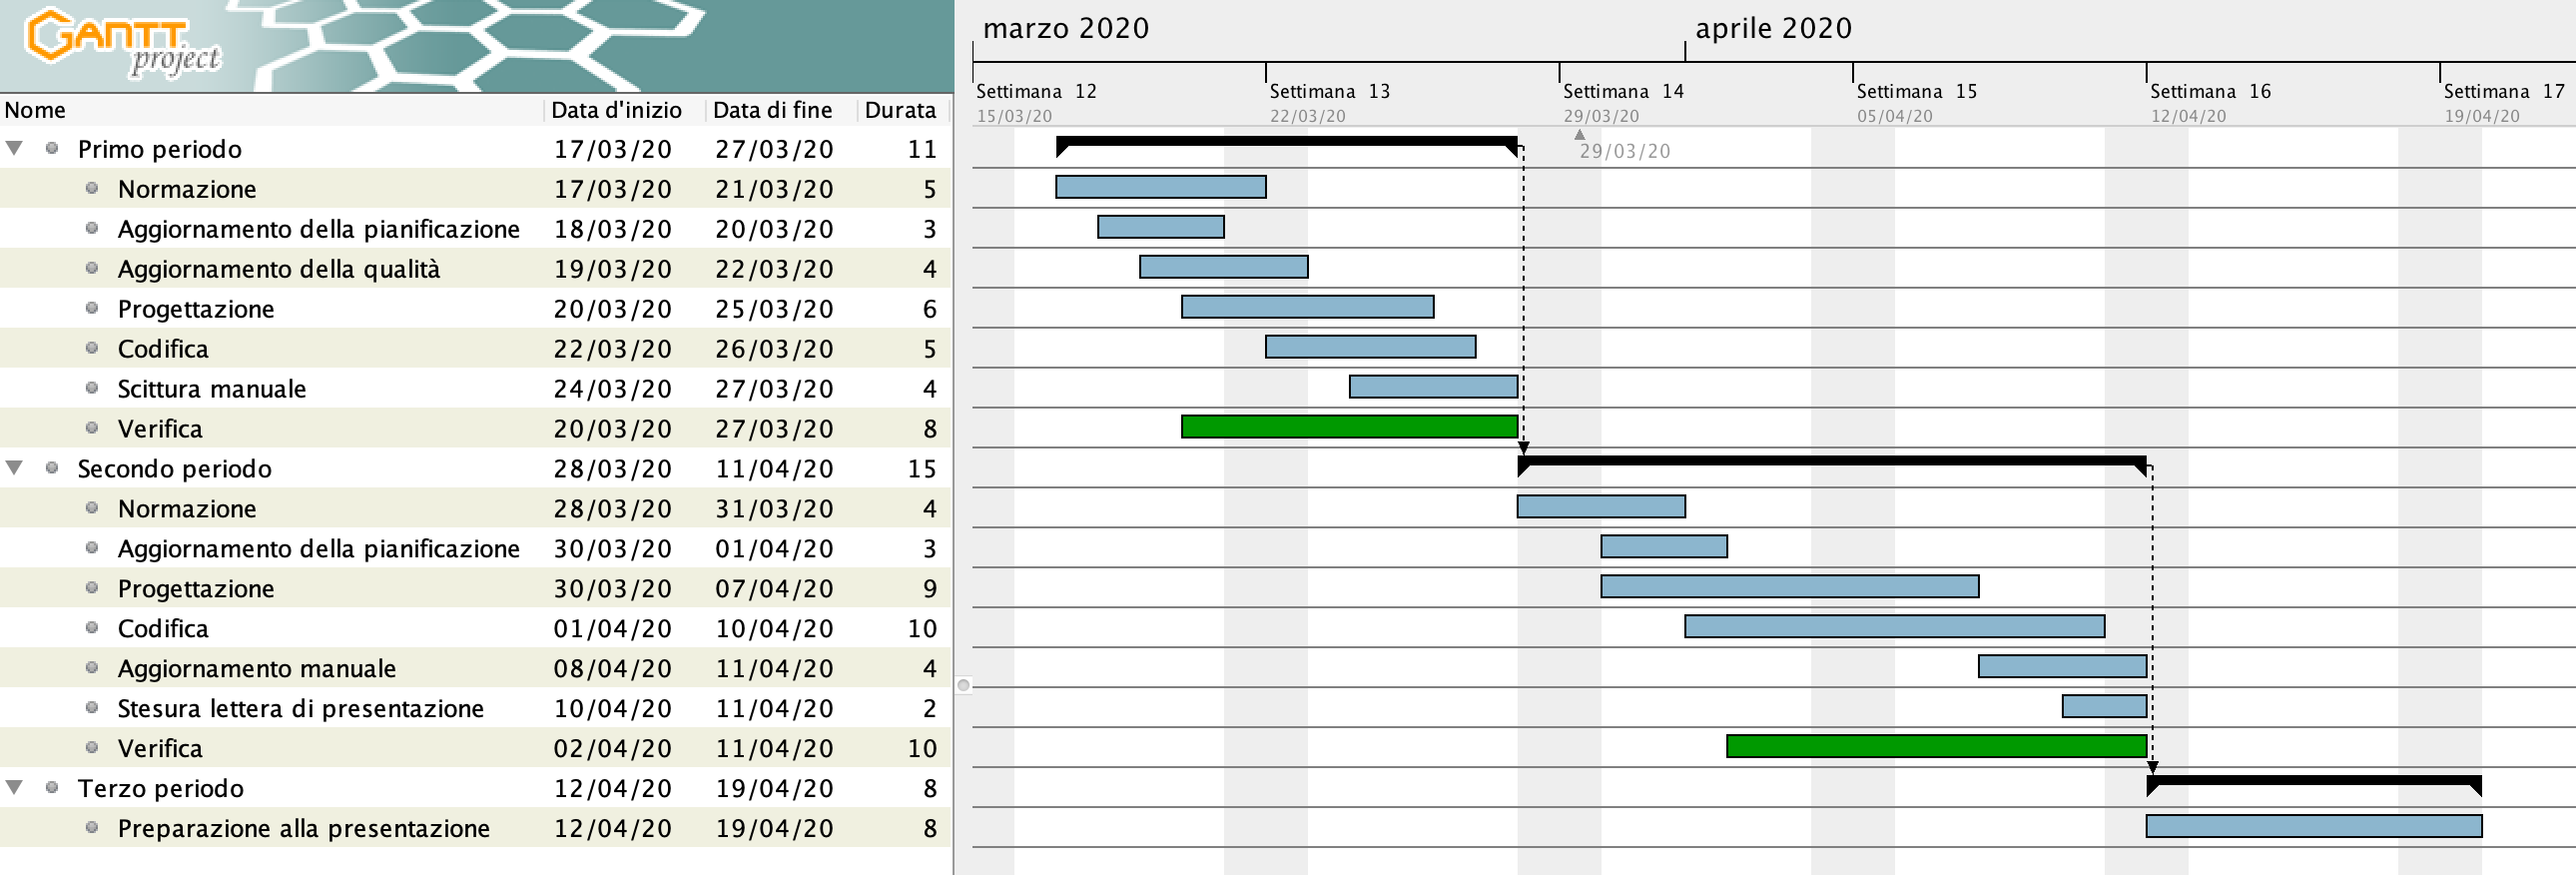
\includegraphics[width=\linewidth]{images/ganttDettaglioCodifica} %TOUPDATE
            \caption{Diagramma di Gantt per l'incremento I}
          \end{figure}		

		\end{landscape}

		% ============================================

		\subsection{Incremento II}
			
			L'incremento II prevede la progettazione di dettaglio e codifica delle componenti software per andare a costituire un \glock{proof of concept}. Si prevede di svolgere quanto segue:
			\begin{itemize}
				\item creazione dell'interfaccia del \glock{gateway} e prima implementazione base;
				\item configurazione della struttura dati con JSON;
				\item implementazione del protocollo di comunicazione con un dispositivo.
			\end{itemize}
			
			\subsubsection{Ruoli attivi}
			
				Durante questa fase è necessaria la presenza dei seguenti ruoli:
				\begin{itemize}
					\item responsabile;
					\item amministratore;
					\item analista;
					\item progettista;
					\item programmatore;
					\item verificatore.
				\end{itemize}
			
			\subsubsection{Periodi e attività}
			
				L'incremento viene svolto in un unico periodo di breve durata.
				
				\paragraph{Unico periodo (dal 2020-02-10 al 2020-02-16)}
				
					\begin{itemize}
						\item \textbf{analisi delle tecnologie:} analisi più approfondita sul funzionamento del \glock{gateway} e sullo sviluppo di un prototipo da utilizzare nel \glock{proof of concept};	
						\item \textbf{progettazione:} progettazione interfaccia del \glock{gateway}, della struttura dati in JSON e del primo protocollo di comunicazione;
						\item \textbf{codifica:} implementazione base del \glock{gateway} e del protocollo di comunicazione con un dispositivo;
						\item \textbf{verifica:} controllo sul funzionamento del \glock{gateway} e sul protocollo di comunicazione con un dispositivo.
					\end{itemize} 			

		\begin{landscape}
          \begin{figure}[H]
            \centering
            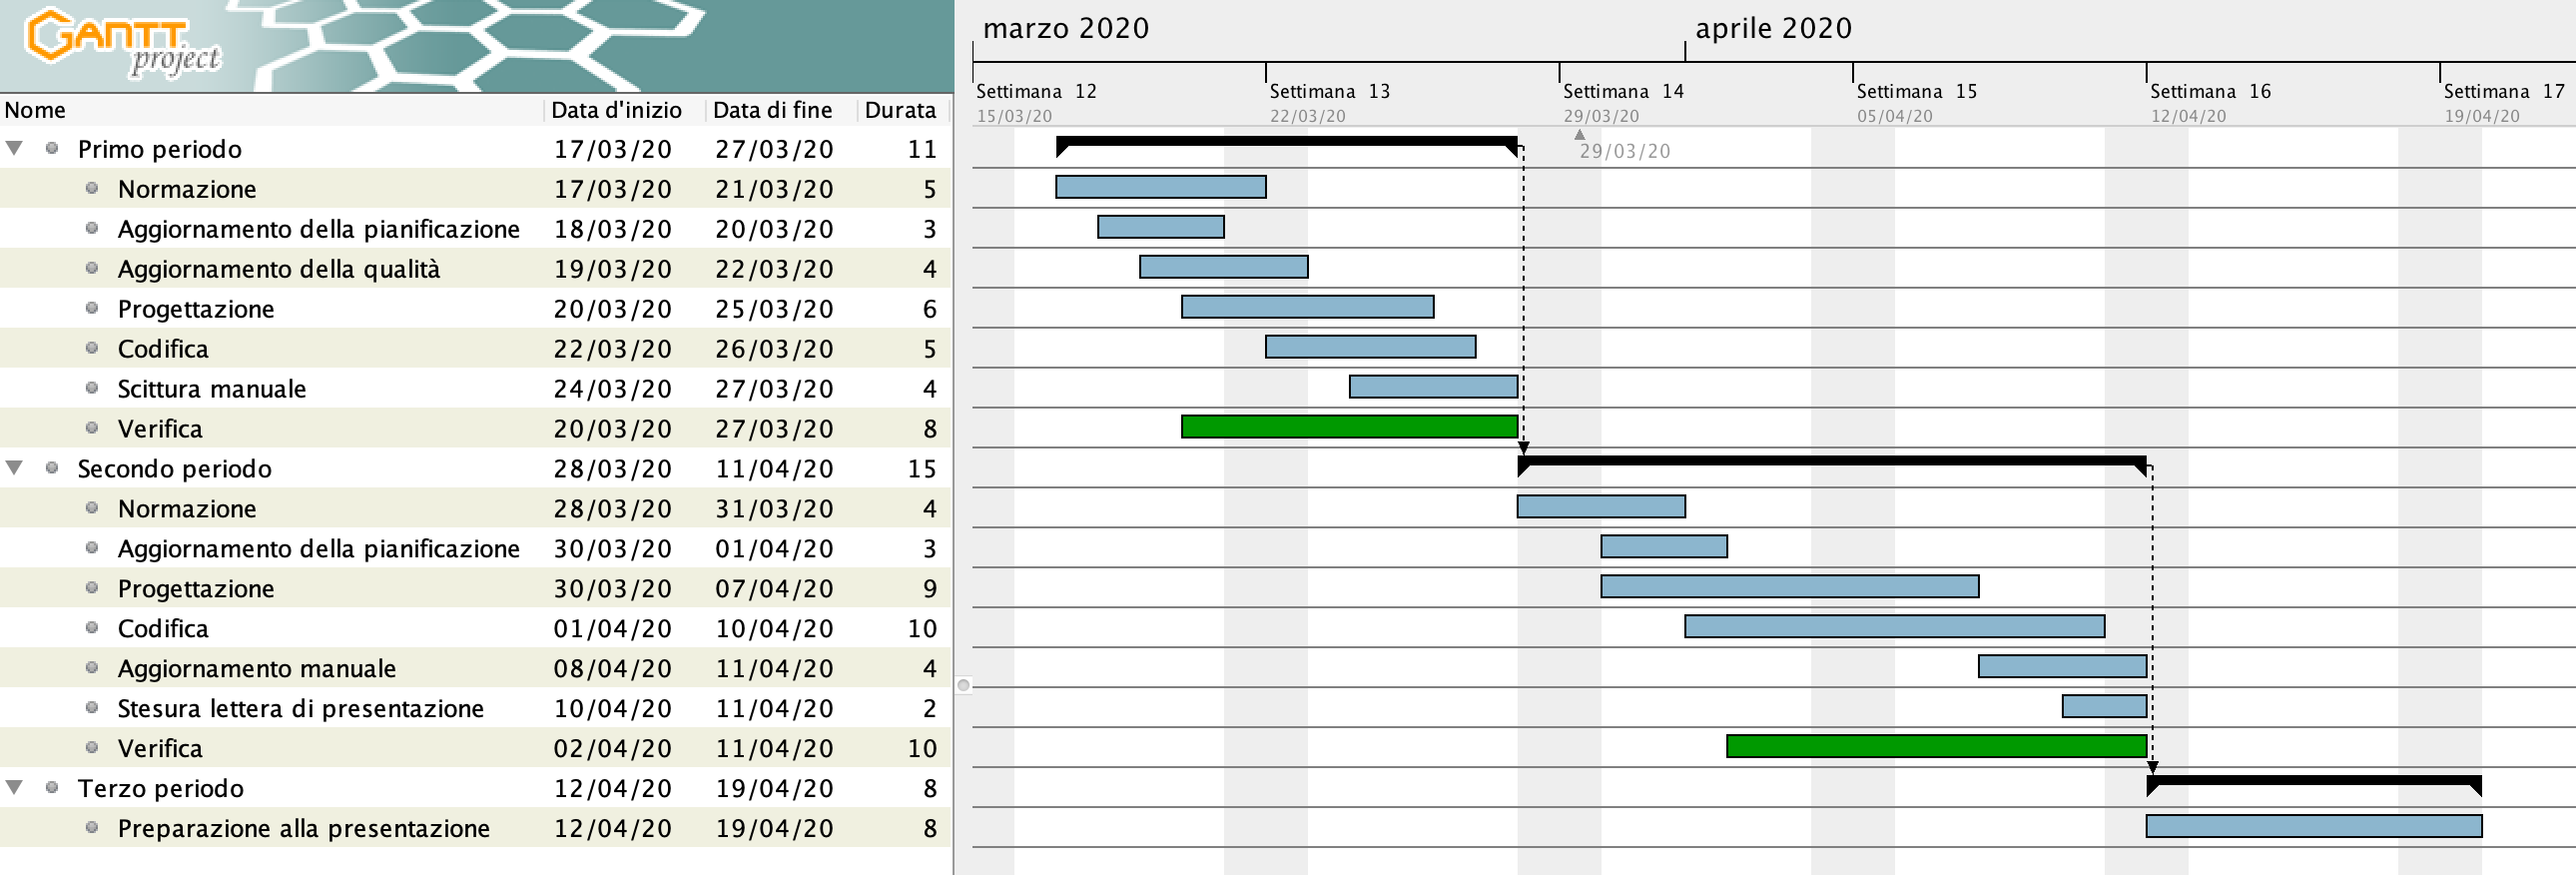
\includegraphics[width=\linewidth]{images/ganttDettaglioCodifica} %TOUPDATE
            \caption{Diagramma di Gantt per l'incremento II}
          \end{figure}		
		\end{landscape}

		% ============================================

		\subsection{Incremento III}
			
			L'incremento III prevede la progettazione di dettaglio e codifica delle componenti software per andare a costituire un \glock{proof of concept}. Si prevede di svolgere quanto segue:
			\begin{itemize}
				\item creazione interfaccia \glock{API};
				\item implementazione operazioni di lettura dei dati con le \glock{API}.
			\end{itemize}
			
			\subsubsection{Ruoli attivi}
			
				Durante questa fase è necessaria la presenza dei seguenti ruoli:
				\begin{itemize}
					\item responsabile;
					\item amministratore;
					\item progettista;
					\item programmatore;
					\item verificatore.
				\end{itemize}
			
			\subsubsection{Periodi e attività}
			
				L'incremento viene svolto in un unico periodo di breve durata.
				
				\paragraph{Unico periodo (dal 2020-02-17 al 2020-02-23)}
				
					\begin{itemize}
						\item \textbf{progettazione:} progettazione interfaccia \glock{API} e relative operazioni di lettura;
						\item \textbf{stesura documentazione API:} stesura della documentazione per le \glock{API}, come richiesto dal capitolato;
						\item \textbf{codifica:} creazione interfaccia \glock{gateway} e implementazioni operazioni di lettura dei dati;
						\item \textbf{verifica:} controllo sul funzionamento del \glock{gateway} e sul protocollo di comunicazione con un dispositivo.
					\end{itemize} 			

		\begin{landscape}
          \begin{figure}[H]
            \centering
            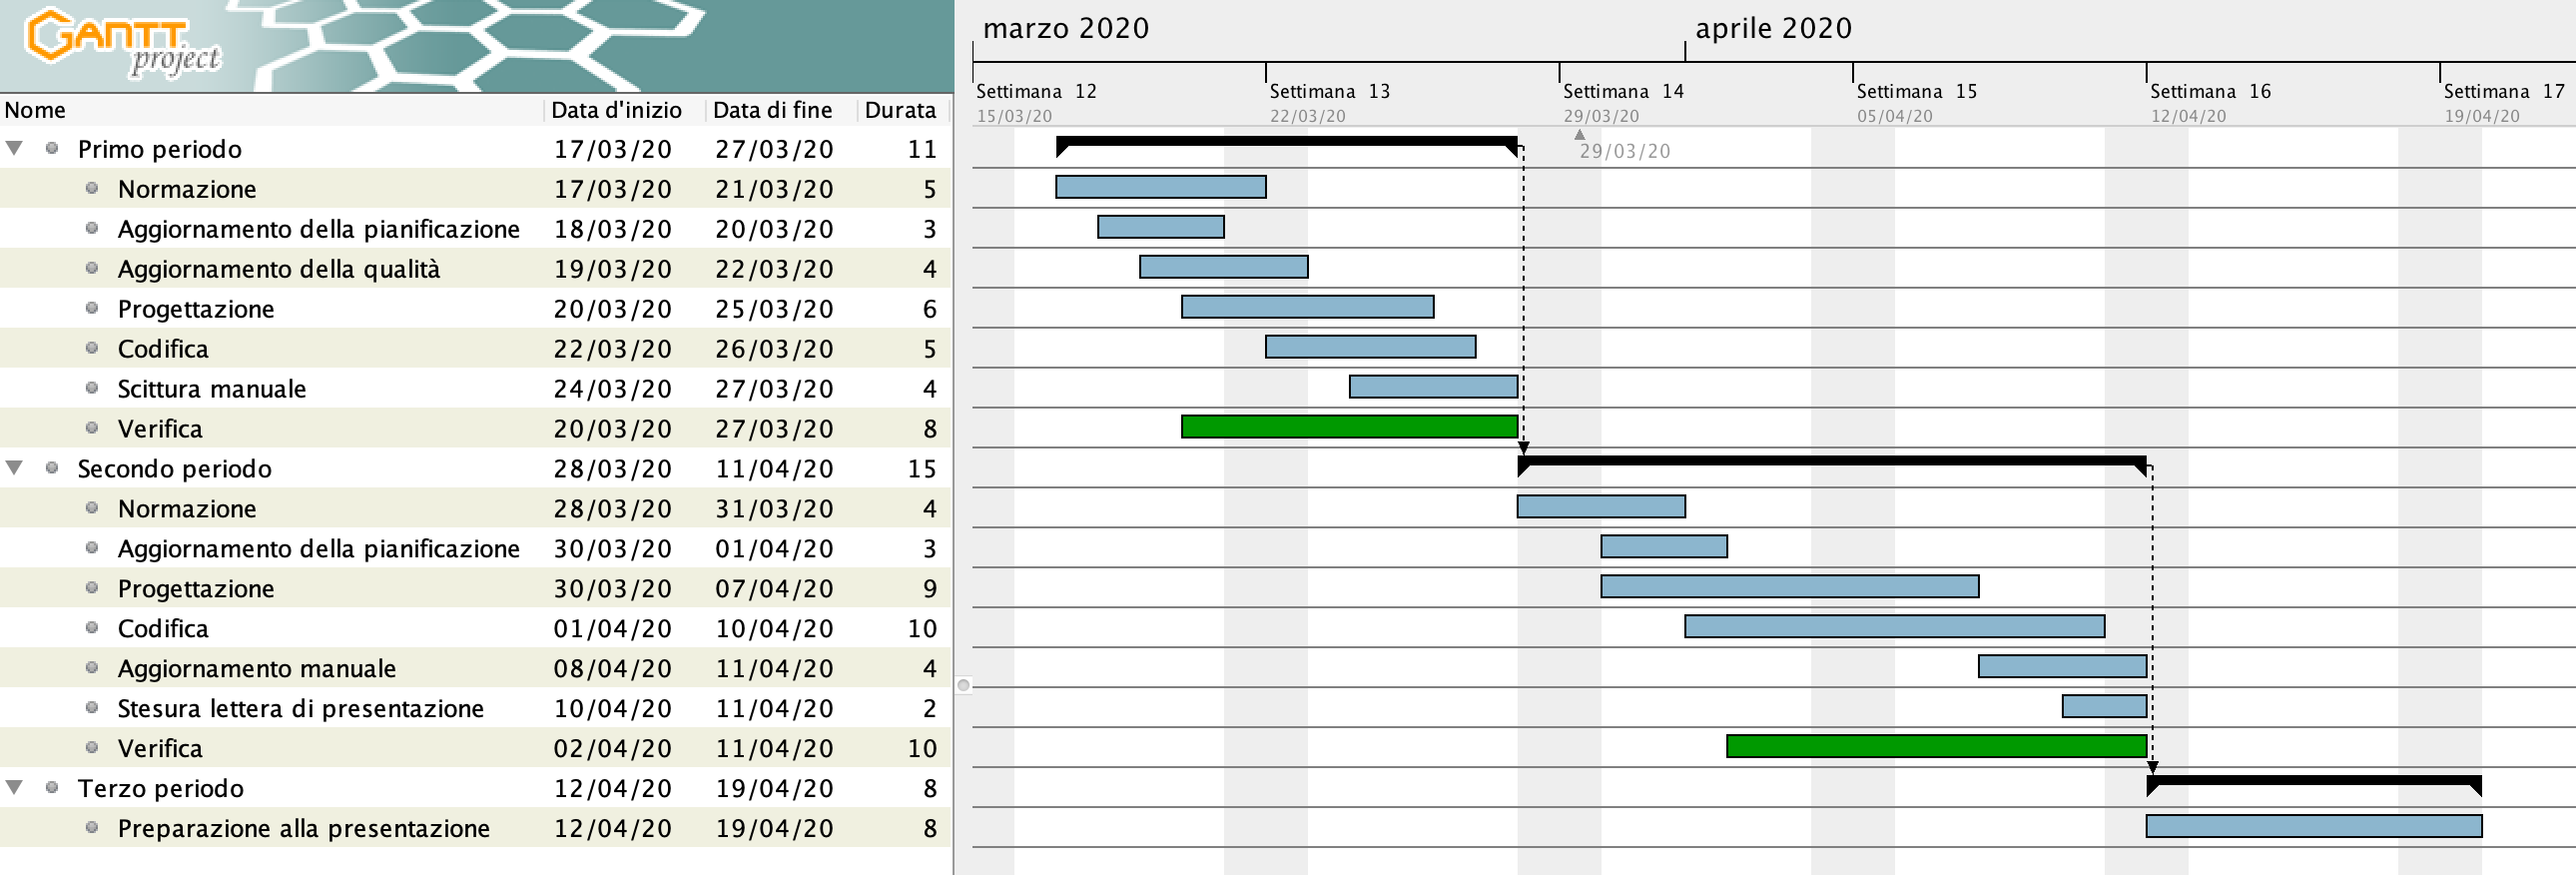
\includegraphics[width=\linewidth]{images/ganttDettaglioCodifica} %TOUPDATE
            \caption{Diagramma di Gantt per l'incremento III}
          \end{figure}		
		\end{landscape}

		% ============================================

		\subsection{Incremento IV}
			
			L'incremento IV prevede la progettazione di dettaglio e codifica delle componenti software per andare a costituire un \glock{proof of concept}. Si prevede di svolgere quanto segue:
			\begin{itemize}
				\item configurazione della struttura base della web app;
				\item reperimento dei dati utilizzati dalla web app dalle \glock{API}.
			\end{itemize}
			Con la fine di questo incremento, si va a costituire un primo \glock{proof of concept} del prodotto che potrà essere mostrato al committente e al proponente.
			
			\subsubsection{Ruoli attivi}
			
				Durante questa fase è necessaria la presenza dei seguenti ruoli:
				\begin{itemize}
					\item responsabile;
					\item amministratore;
					\item analista;
					\item progettista;
					\item programmatore;
					\item verificatore.
				\end{itemize}
			
			\subsubsection{Periodi e attività}
			
				L'incremento viene svolto in un unico periodo di breve durata.
				
				\paragraph{Unico periodo (dal 2020-02-24 al 2020-03-01)}
				
					\begin{itemize}
						\item \textbf{analisi delle tecnologie:} analisi sulla sintassi da usare nelle \glock{API} e sulle funzionalità necessarie da implementare;	
						\item \textbf{progettazione:} progettazione della struttura base del sito con reperimento dati per mezzo delle \glock{API} per le operazioni attualmente implementate;
						\item \textbf{codifica:} creazione della struttura base del sito con un accenno alla \glock{user interface} e reperimento dei dati tramite \glock{API};
						\item \textbf{verifica:} controllo sul funzionamento dei dati recuperati dalla web app e sull'utilizzo iniziale in modalità mobile e desktop.
					\end{itemize} 			

		\begin{landscape}
          \begin{figure}[H]
            \centering
            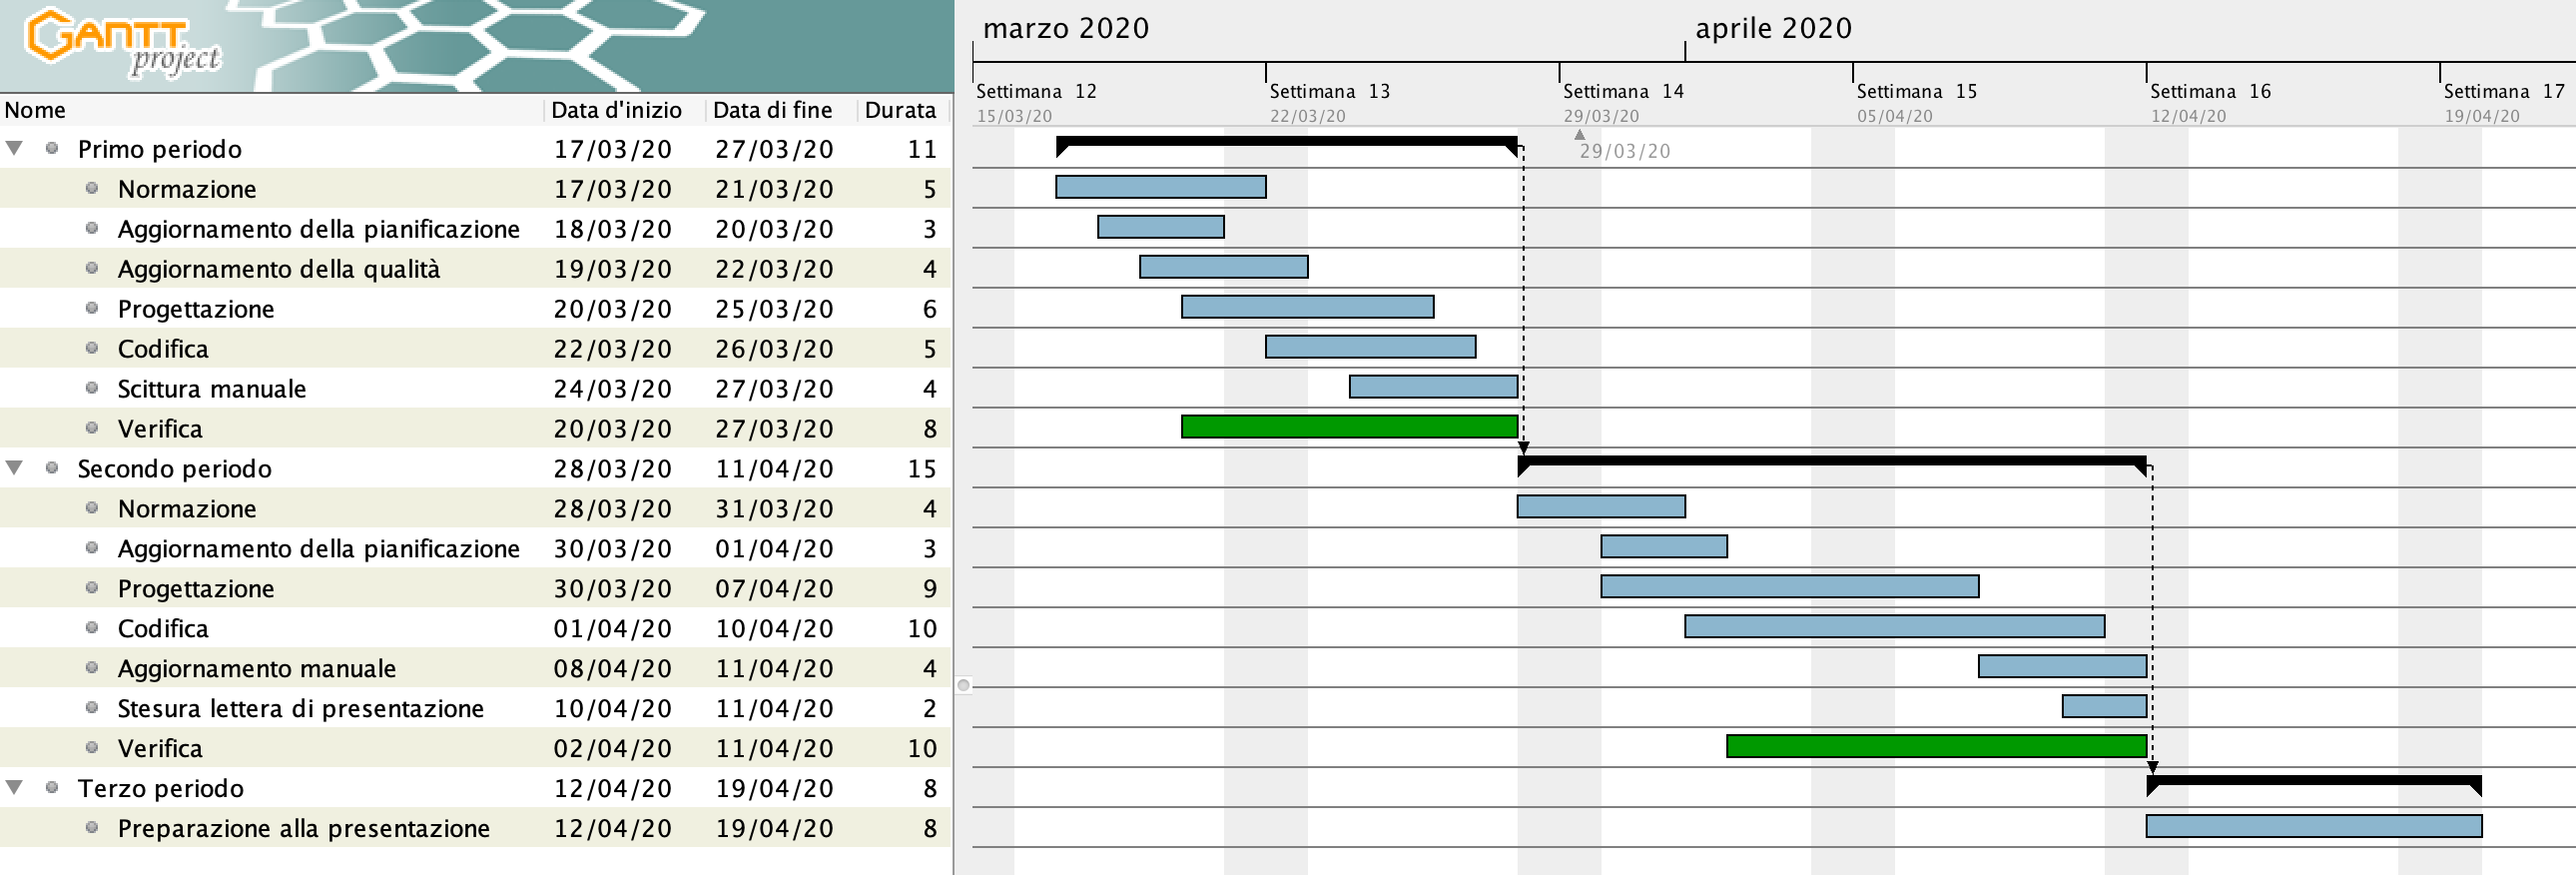
\includegraphics[width=\linewidth]{images/ganttDettaglioCodifica} %TOUPDATE
            \caption{Diagramma di Gantt per l'incremento IV}
          \end{figure}		
		\end{landscape}

		% ============================================

		\subsection{Incremento V}
			
			L'incremento V prevede la progettazione di dettaglio e codifica delle componenti software e la preparazione di una presentazione per le tecnologie utilizzate. A livello software, si prevede di svolgere quanto segue:
			\begin{itemize}
				\item implementazione della configurazione dinamica per un \glock{gateway}.
			\end{itemize}
			
			\subsubsection{Ruoli attivi}
			
				Durante questa fase è necessaria la presenza dei seguenti ruoli:
				\begin{itemize}
					\item responsabile;
					\item amministratore;
					\item progettista;
					\item programmatore;
					\item verificatore.
				\end{itemize}
			
			\subsubsection{Periodi e attività}
			
				L'incremento viene svolto in un unico periodo di breve durata.
				
				\paragraph{Unico periodo (dal 2020-03-02 al 2020-03-08)}
				
					\begin{itemize}
						\item \textbf{presentazione:} inizio creazione slides per la presentazione della \textit{technology baseline};
						\item \textbf{progettazione:} progettazione della configurazione dinamica del \glock{gateway};
						\item \textbf{codifica:} implementazione della funzionalità di aggiornamento automatico della configurazione per il \glock{gateway};
						\item \textbf{verifica software:} controllo sulla funzionalità delle componenti modificate.
						% \item \textbf{stesura:} continuazione del \textit{manuale di manutenzione}, integrazione della componente \glock{gateway};
						% \item \textbf{verifica documenti:} verifica delle sezioni aggiunte nel documento modificato.
					\end{itemize} 			

		\begin{landscape}
          \begin{figure}[H]
            \centering
            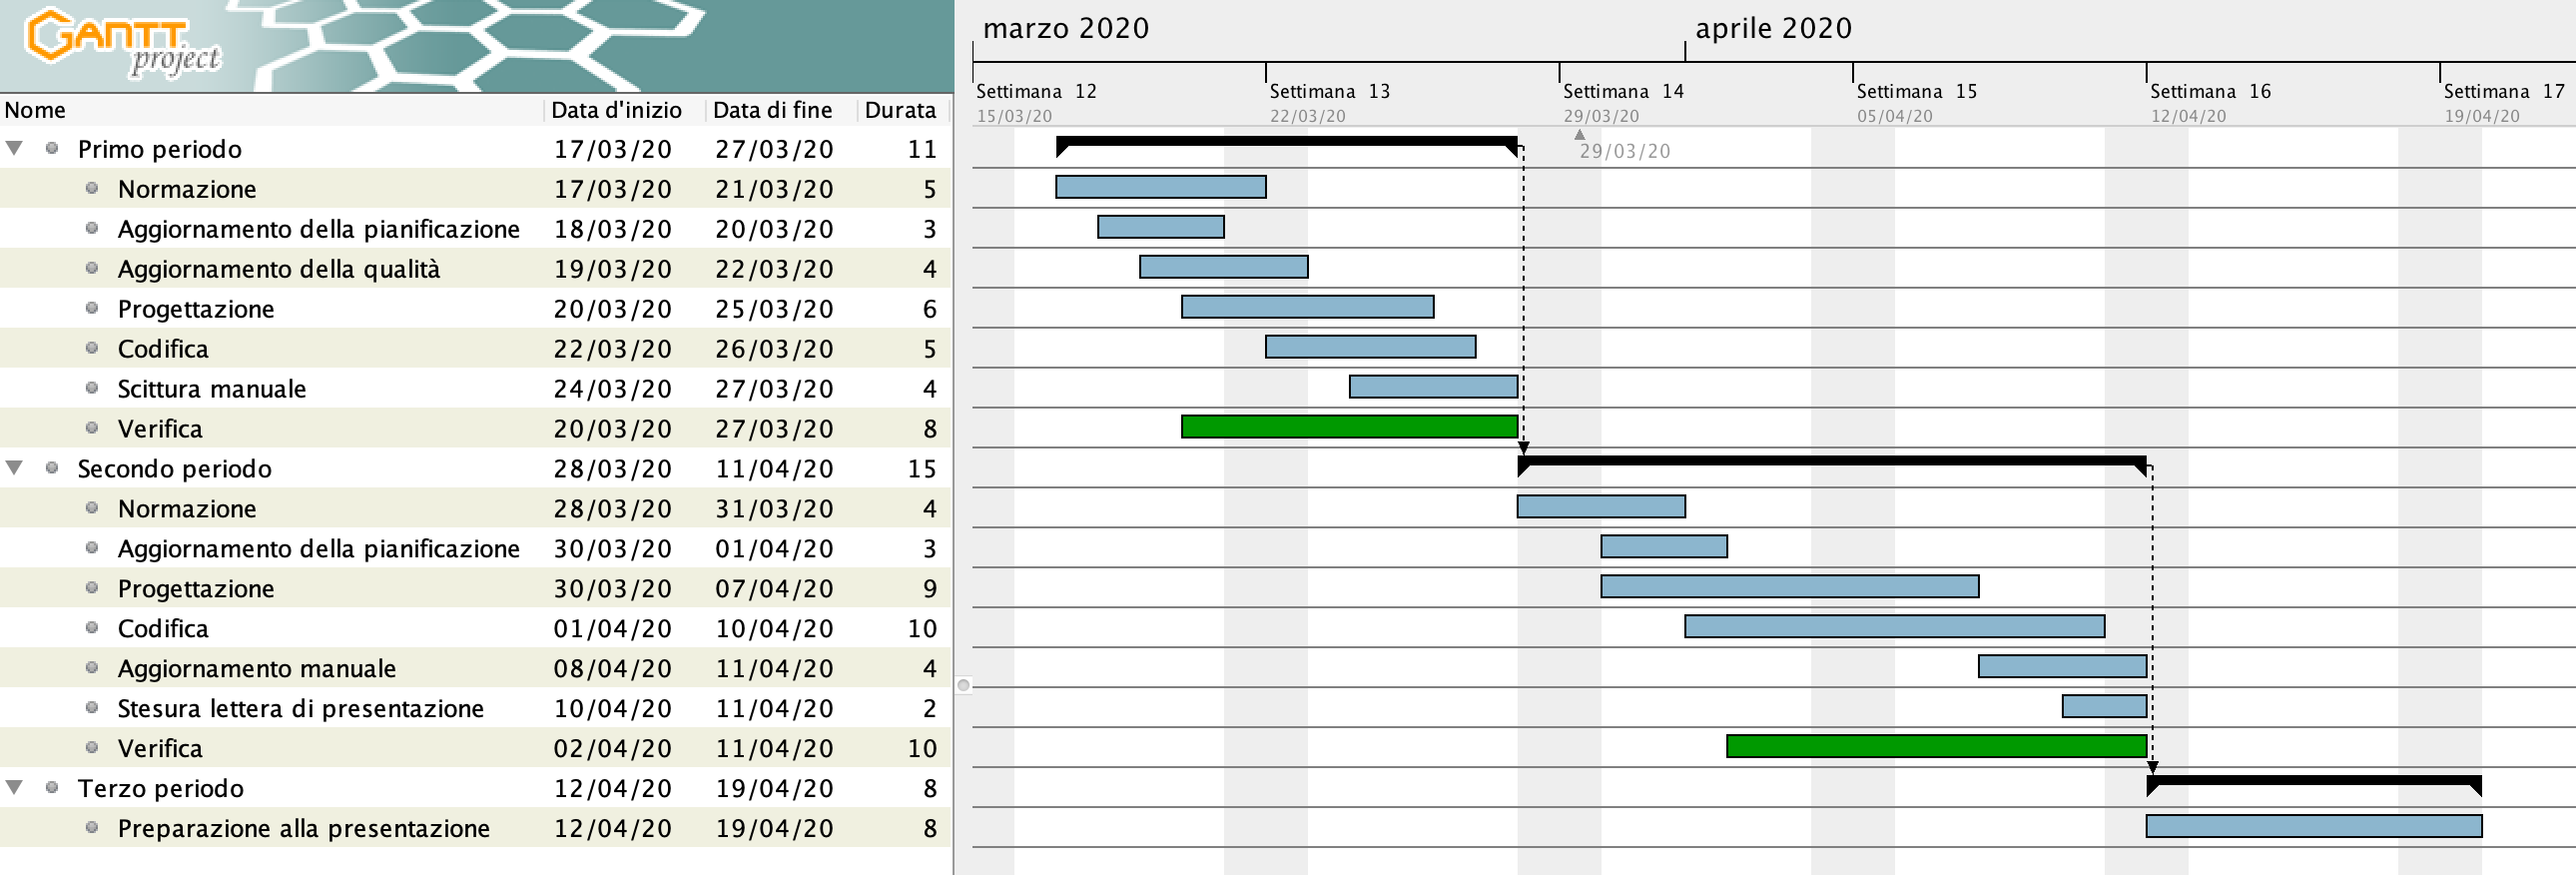
\includegraphics[width=\linewidth]{images/ganttDettaglioCodifica} %TOUPDATE
            \caption{Diagramma di Gantt per l'incremento V}
          \end{figure}		
		\end{landscape}

		% ============================================

		\subsection{Incremento VI}
			
			L'incremento VI prevede la progettazione di dettaglio e codifica delle componenti software e la preparazione di una presentazione per le tecnologie utilizzate. Si prevede di svolgere quanto segue:
			\begin{itemize}
				\item implementazione dei database (relazionale e non relazionale);
				\item configurazione della comunicazione dei database con Kafka.
			\end{itemize}
			
			\subsubsection{Ruoli attivi}
			
				Durante questa fase è necessaria la presenza dei seguenti ruoli:
				\begin{itemize}
					\item responsabile;
					\item amministratore;
					\item analista;
					\item progettista;
					\item programmatore;
					\item verificatore.
				\end{itemize}
			
			\subsubsection{Periodi e attività}
			
				L'incremento viene svolto in un unico periodo di breve durata.
				
				\paragraph{Unico periodo (dal 2020-03-09 al 2020-03-15)}
				
					\begin{itemize}
						\item \textbf{analisi sulle tecnologie:} analisi delle funzionalità dei database nel dettaglio;
						\item \textbf{presentazione:} conclusione creazione slides per la presentazione della \textit{technology baseline};
						\item \textbf{progettazione:} progettazione dei database;
						\item \textbf{creazione diagramma ER:} realizzazione di un diagramma ER per il database relazionale, come richiesto dal capitolato;
						\item \textbf{creazione struttura database:} stesura della struttura del database non relazionale, come richiesto dal capitolato;
						\item \textbf{codifica:} implementazione dei database sulla base della loro progettazione;
						\item \textbf{verifica:} controllo della correttezza con i relativi linguaggi utilizzati.
					\end{itemize} 			

		\begin{landscape}
          \begin{figure}[H]
            \centering
            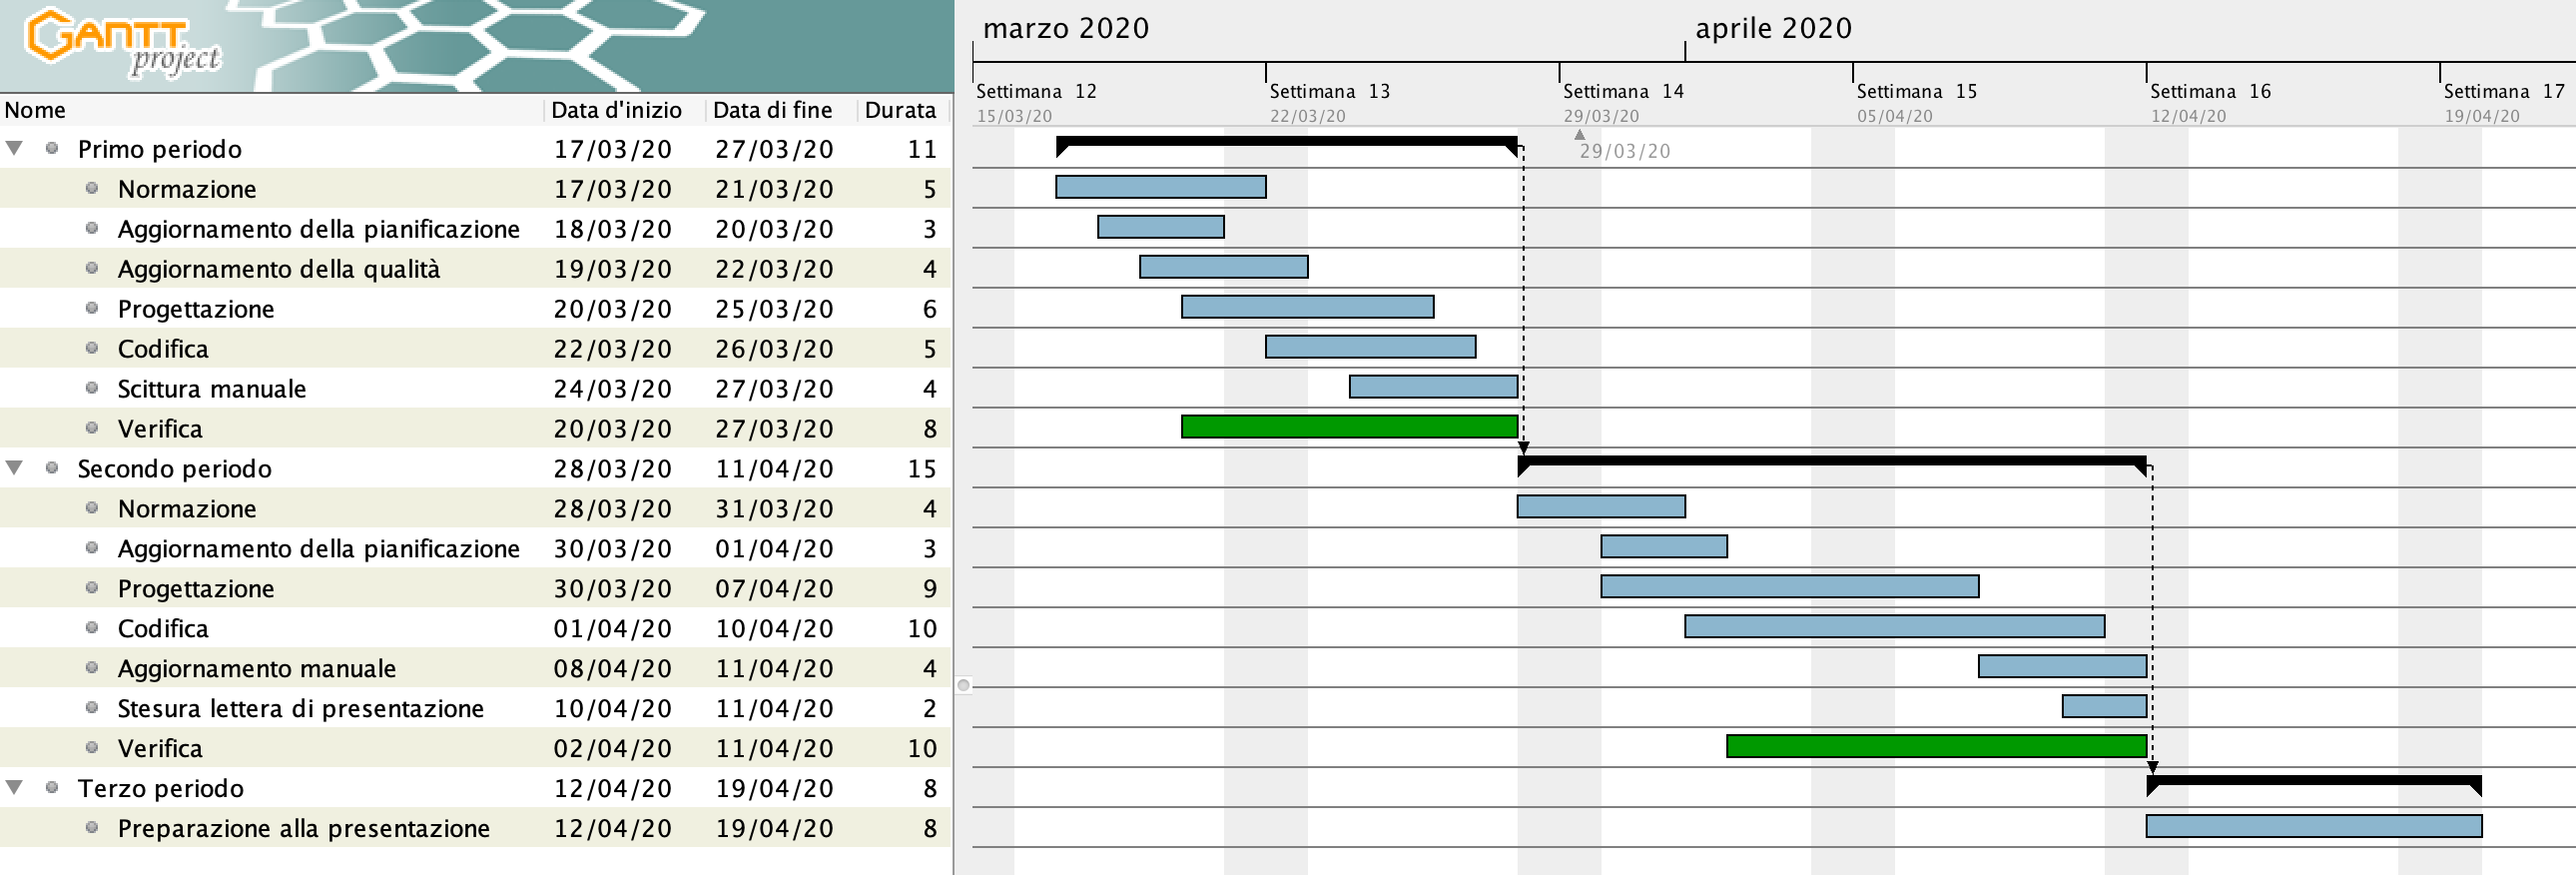
\includegraphics[width=\linewidth]{images/ganttDettaglioCodifica} %TOUPDATE
            \caption{Diagramma di Gantt per l'incremento VI}
          \end{figure}		
		\end{landscape}

		% ============================================

		\subsection{Incremento VII}
			
			L'incremento VII prevede la progettazione di dettaglio e codifica delle componenti software. Si prevede di svolgere quanto segue:
			\begin{itemize}
				\item implementazione base \glock{bot Telegram} per la ricezione di avvisi;
				\item configurazione del \glock{bot Telegram} con le \glock{API};
				\item implementazione del login per la web app.
			\end{itemize}
			
			\subsubsection{Ruoli attivi}
			
				Durante questa fase è necessaria la presenza dei seguenti ruoli:
				\begin{itemize}
					\item responsabile;
					\item amministratore;
					\item progettista;
					\item programmatore;
					\item verificatore.
				\end{itemize}
			
			\subsubsection{Periodi e attività}
			
				L'incremento viene svolto in un unico periodo di breve durata.
				
				\paragraph{Unico periodo (dal 2020-03-16 al 2020-03-22)}
				
					\begin{itemize}
						\item \textbf{progettazione:} 
						\begin{itemize}
							\item progettazione del \glock{bot Telegram} per la ricezione avvisi e interazioni base dall'applicazione alle \glock{API}; 
							\item progettazione della schermata di accesso della web app;
						\end{itemize}
						\item \textbf{codifica:} 
						\begin{itemize}
							\item implementazione base del \glock{bot Telegram}, come descritto nella progettazione; 
							\item implementazione della schermata di login del sito web e della parte privata e pubblica del sito;
						\end{itemize}
						\item \textbf{verifica software:} controllo delle nuove funzionalità tali per cui soddisfino i requisiti predisposti;
						\item \textbf{stesura:} continuazione del \textit{manuale di manutenzione}, integrazione delle componenti per \glock{Telegram} e per l'accesso alla web app;
						\item \textbf{verifica documenti:} verifica delle sezioni aggiunte nel documento modificato.
					\end{itemize} 			

		\begin{landscape}
          \begin{figure}[H]
            \centering
            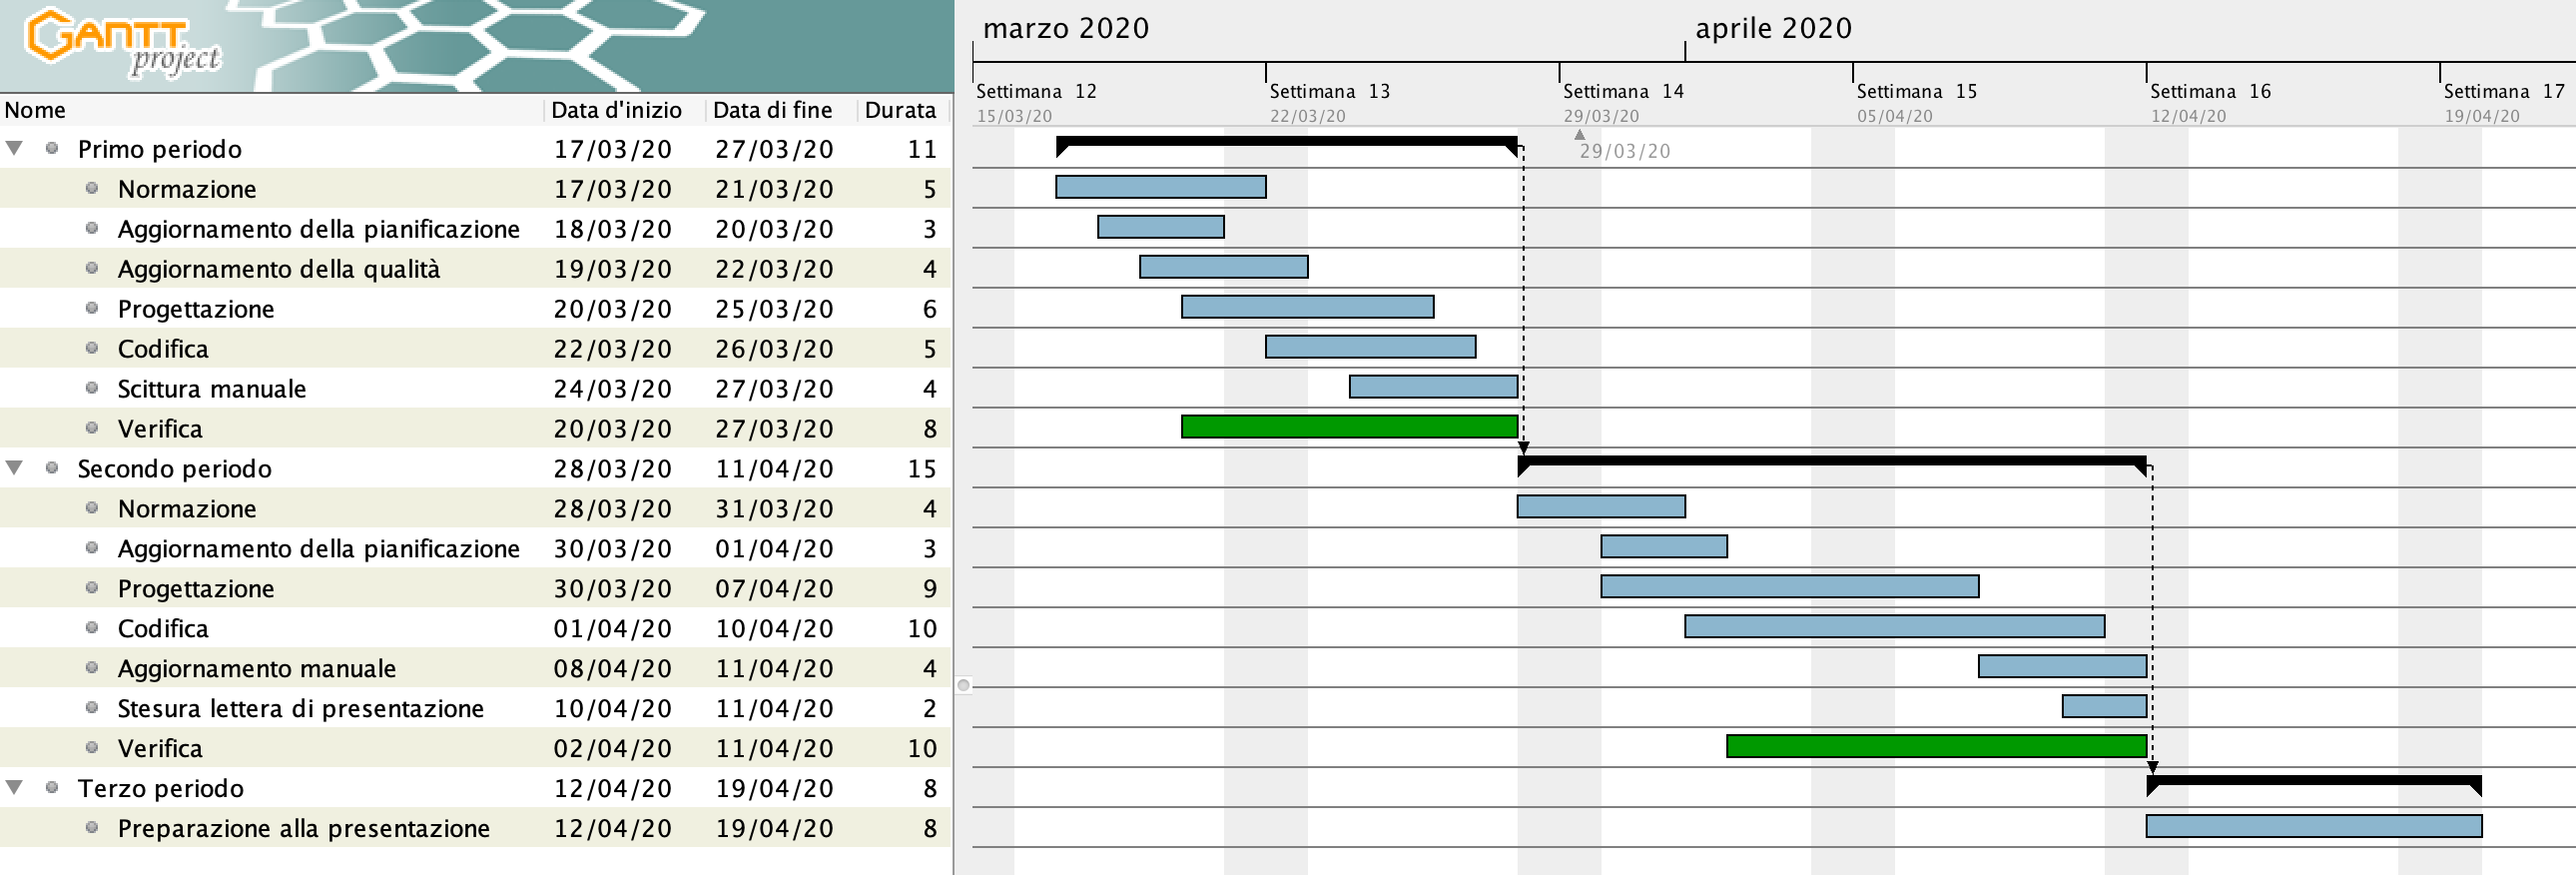
\includegraphics[width=\linewidth]{images/ganttDettaglioCodifica} %TOUPDATE
            \caption{Diagramma di Gantt per l'incremento VII}
          \end{figure}		
		\end{landscape}

		% ============================================

		\subsection{Incremento VIII}
			
			L'incremento VIII prevede la progettazione di dettaglio e codifica delle componenti software. Si prevede di svolgere quanto segue:
			\begin{itemize}
				\item implementazione dei grafici per la web app.
			\end{itemize}
			
			\subsubsection{Ruoli attivi}
			
				Durante questa fase è necessaria la presenza dei seguenti ruoli:
				\begin{itemize}
					\item responsabile;
					\item amministratore;
					\item progettista;
					\item programmatore;
					\item verificatore.
				\end{itemize}
			
			\subsubsection{Periodi e attività}
			
				L'incremento viene svolto in un unico periodo di breve durata.
				
				\paragraph{Unico periodo (dal 2020-03-23 al 2020-03-29)}
				
					\begin{itemize}
						\item \textbf{progettazione:} progettazione dei grafici per la web app;
						\item \textbf{codifica:} implementazione dei grafici e delle funzioni utili per la generazione dei grafici in tempo reale e delle correlazioni;
						\item \textbf{verifica software:} controllo delle nuove funzionalità tali per cui soddisfino i requisiti predisposti;
						\item \textbf{stesura:} continuazione del \textit{manuale di manutenzione}, integrazione delle funzioni per la generazione dei grafici e delle correlazioni disponibili;
						\item \textbf{verifica documenti:} verifica delle sezioni aggiunte nel documento modificato.
					\end{itemize} 			

		\begin{landscape}
          \begin{figure}[H]
            \centering
            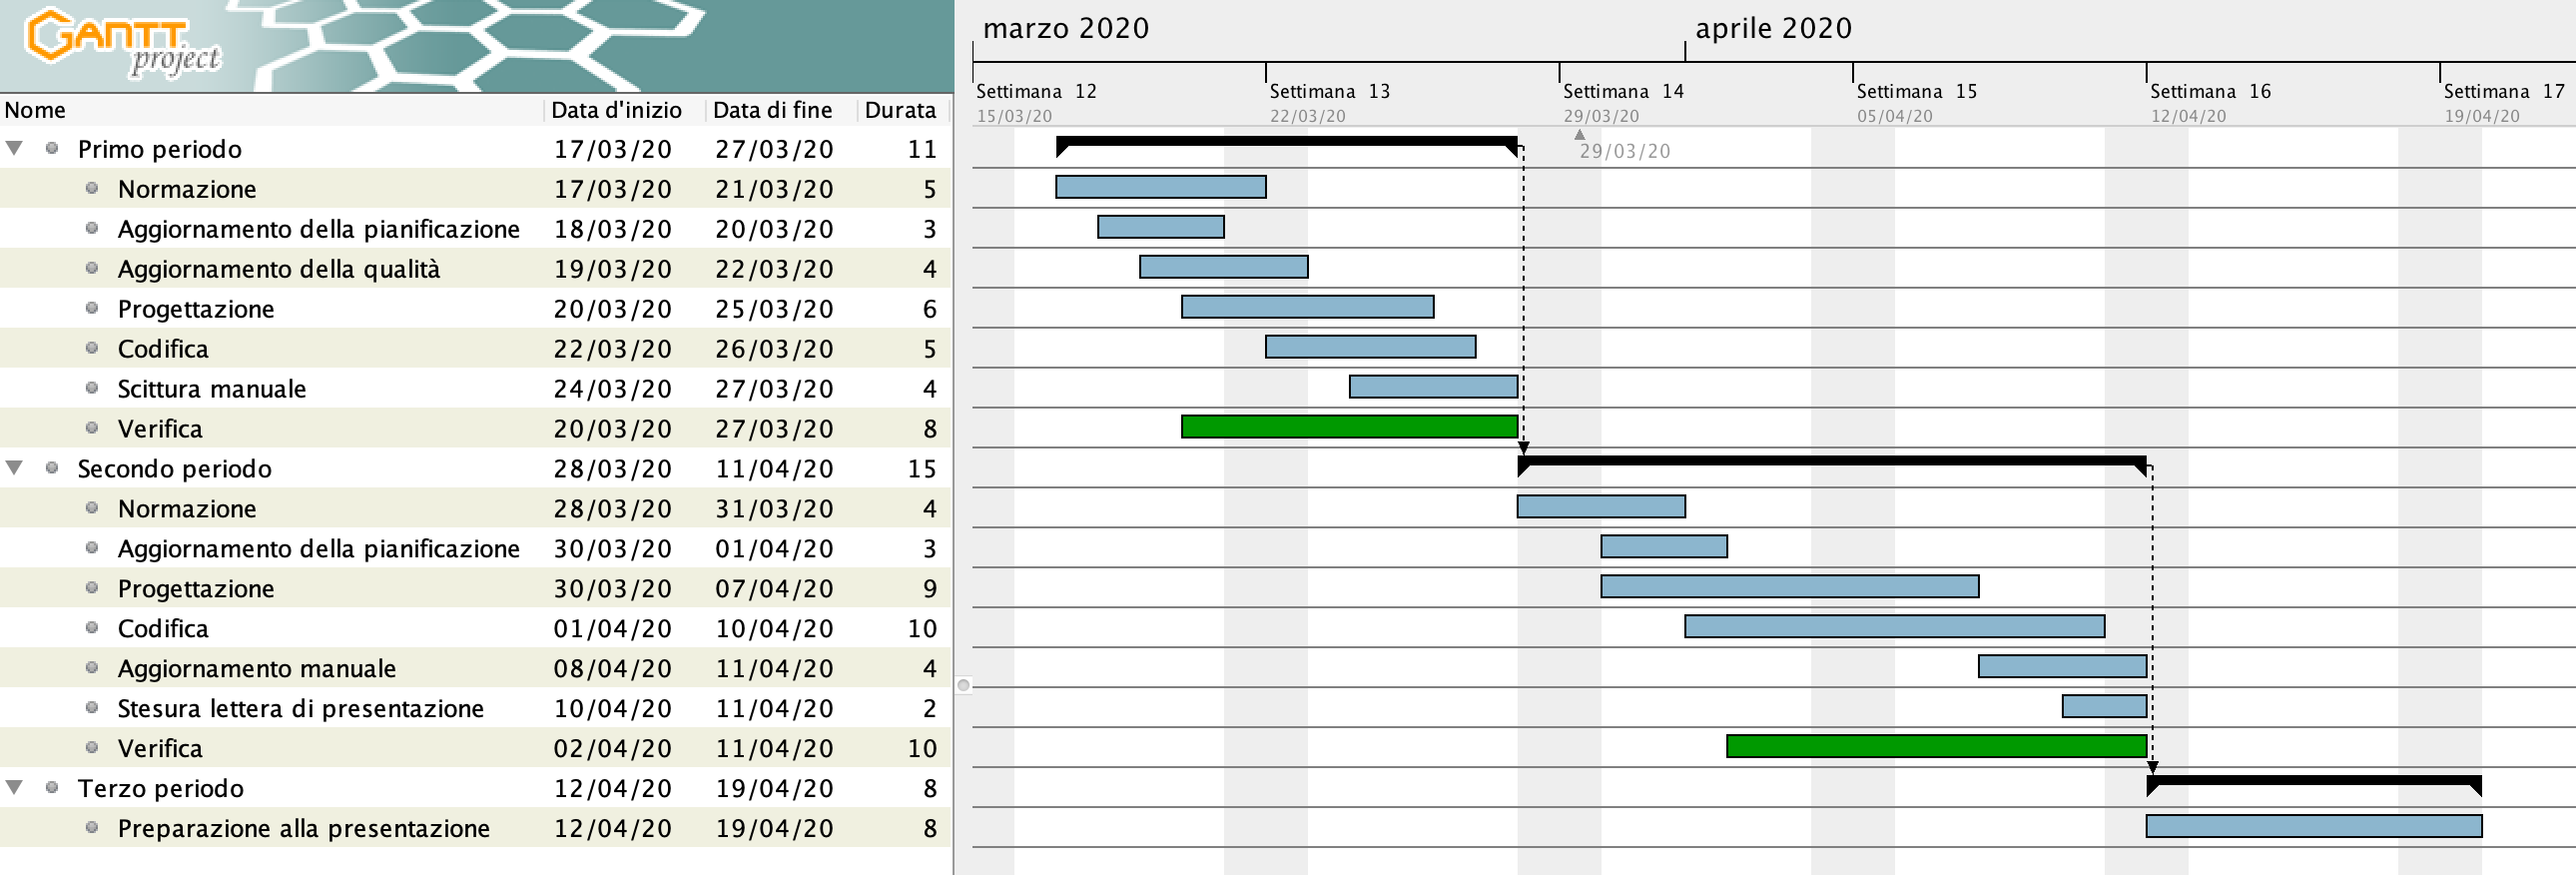
\includegraphics[width=\linewidth]{images/ganttDettaglioCodifica} %TOUPDATE
            \caption{Diagramma di Gantt per l'incremento VIII}
          \end{figure}		
		\end{landscape}

		% ============================================

		\subsection{Incremento IX}
			
			L'incremento IX prevede la progettazione di dettaglio e codifica delle componenti software. Si prevede di svolgere quanto segue:
			\begin{itemize}
				\item implementazione della parte utente per la web app.
			\end{itemize}
			
			\subsubsection{Ruoli attivi}
			
				Durante questa fase è necessaria la presenza dei seguenti ruoli:
				\begin{itemize}
					\item responsabile;
					\item amministratore;
					\item progettista;
					\item programmatore;
					\item verificatore.
				\end{itemize}
			
			\subsubsection{Periodi e attività}
			
				L'incremento viene svolto in un unico periodo di breve durata.
				
				\paragraph{Unico periodo (dal 2020-03-30 al 2020-04-05)}
				
					\begin{itemize}
						\item \textbf{progettazione:} progettazione della parte utente per la web app;
						\item \textbf{codifica:} implementazione della parte utente con tutte le relative sezioni disponibili;
						\item \textbf{verifica software:} controllo delle nuove funzionalità tali per cui soddisfino i requisiti predisposti;
						\item \textbf{stesura:} 
							\begin{itemize}
								\item \textit{manuale di manutenzione:} integrazione delle funzioni disponibili agli utenti;
								\item \textit{manuale utente:} descrizione delle funzionalità per un utente;
							\end{itemize}
						\item \textbf{verifica documenti:} verifica delle sezioni aggiunte nei documenti modificati.
					\end{itemize} 			

		\begin{landscape}
          \begin{figure}[H]
            \centering
            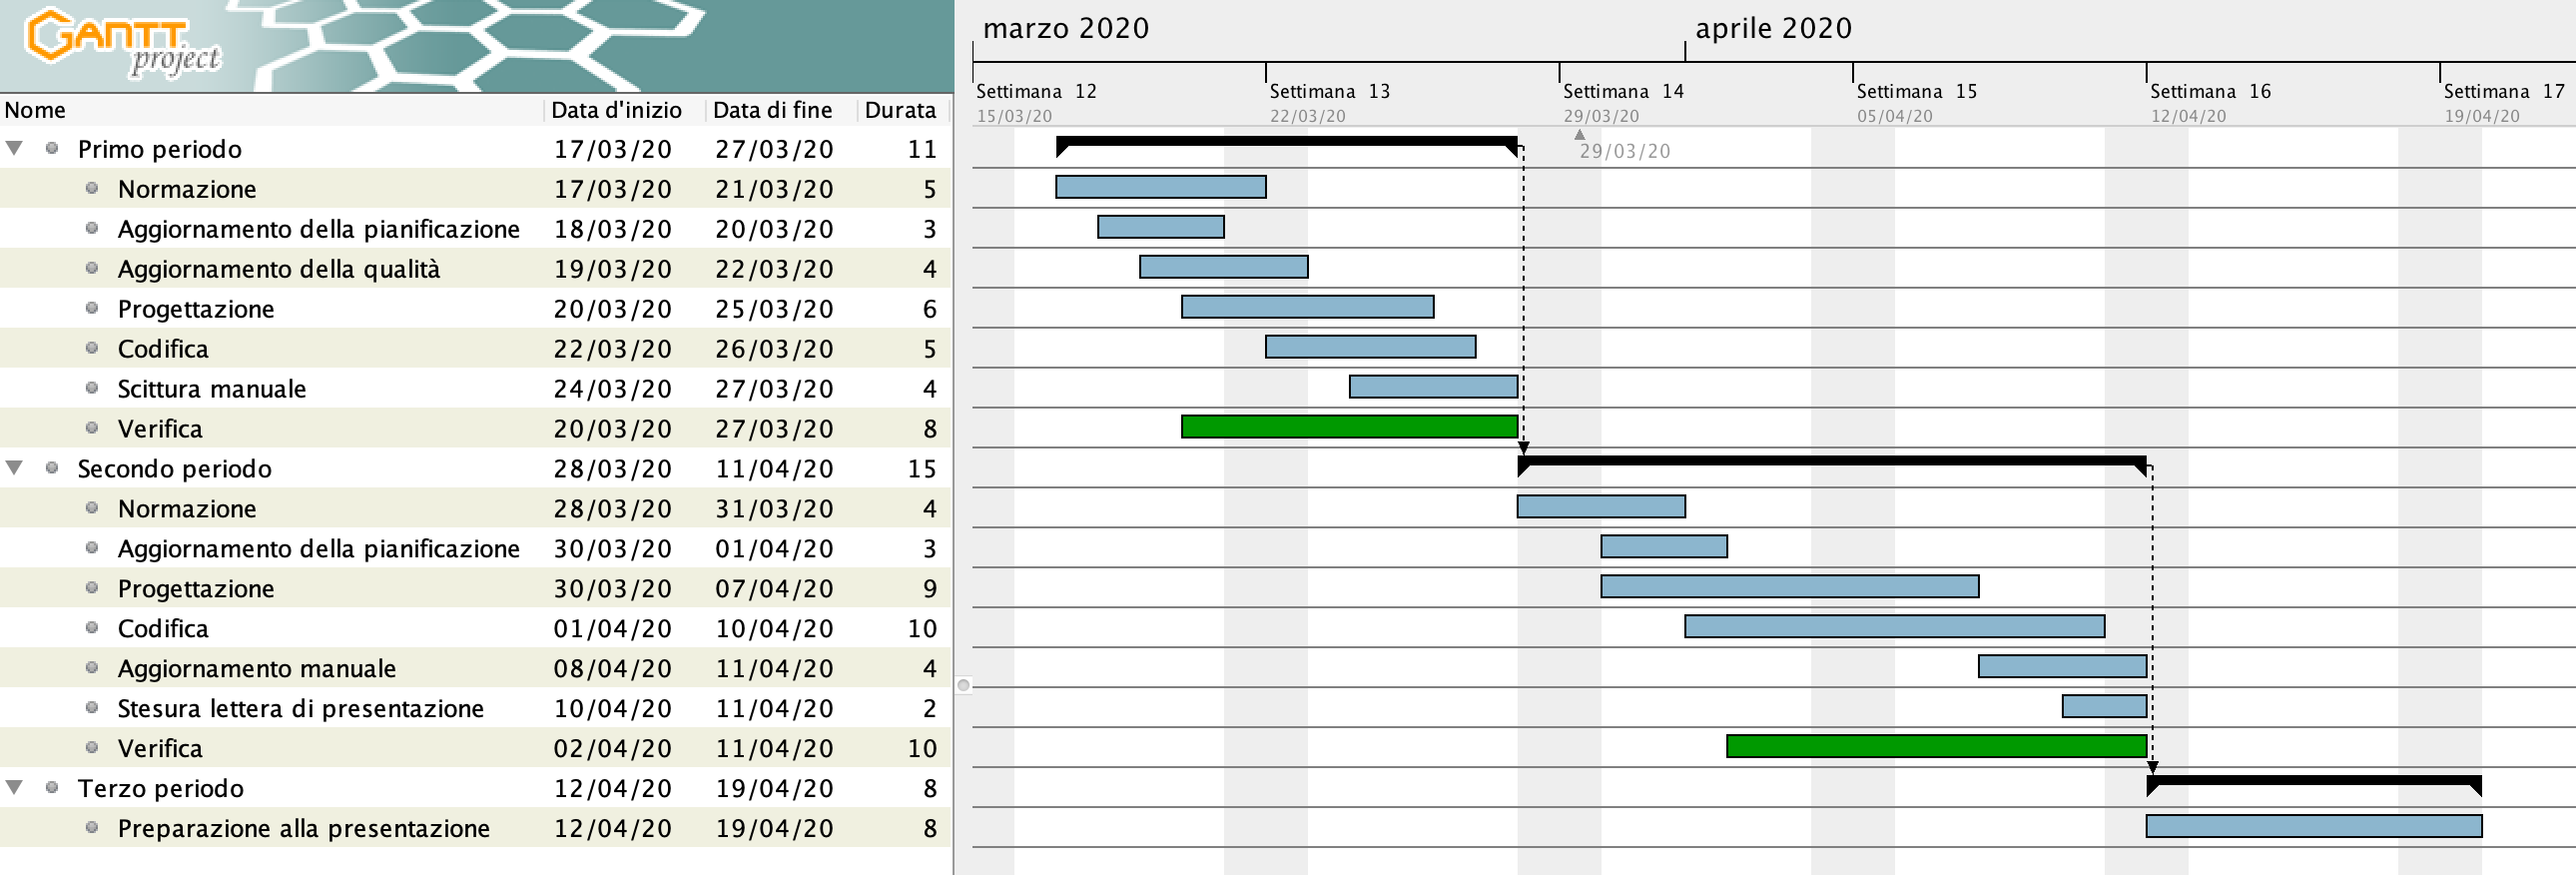
\includegraphics[width=\linewidth]{images/ganttDettaglioCodifica} %TOUPDATE
            \caption{Diagramma di Gantt per l'incremento IX}
          \end{figure}		
		\end{landscape}

		% ============================================

		\subsection{Incremento X}
			
			L'incremento X prevede la progettazione di dettaglio e codifica delle componenti software. Si prevede di svolgere quanto segue:
			\begin{itemize}
				\item implementazione della moderazione per gli enti nella web app.
			\end{itemize}
			
			\subsubsection{Ruoli attivi}
			
				Durante questa fase è necessaria la presenza dei seguenti ruoli:
				\begin{itemize}
					\item responsabile;
					\item amministratore;
					\item progettista;
					\item programmatore;
					\item verificatore.
				\end{itemize}
			
			\subsubsection{Periodi e attività}
			
				L'incremento viene svolto in un unico periodo di breve durata.
				
				\paragraph{Unico periodo (dal 2020-04-06 al 2020-04-12)}
				
					\begin{itemize}
						\item \textbf{progettazione:} progettazione della moderazione ente per la web app;
						\item \textbf{codifica:} implementazione della moderazione ente con tutte le relative funzioni per gli utenti;
						\item \textbf{verifica software:} controllo delle nuove funzionalità tali per cui soddisfino i requisiti predisposti;
						\item \textbf{stesura:}
						\begin{itemize}
							\item \textit{manuale di manutenzione:} integrazione delle funzioni disponibili per i moderatori enti;
							\item \textit{manuale utente:} descrizione delle funzionalità per un moderatore ente;
						\end{itemize}
						\item \textbf{verifica documenti:} verifica delle sezioni aggiunte nei documenti modificati.
					\end{itemize} 			

		\begin{landscape}
          \begin{figure}[H]
            \centering
            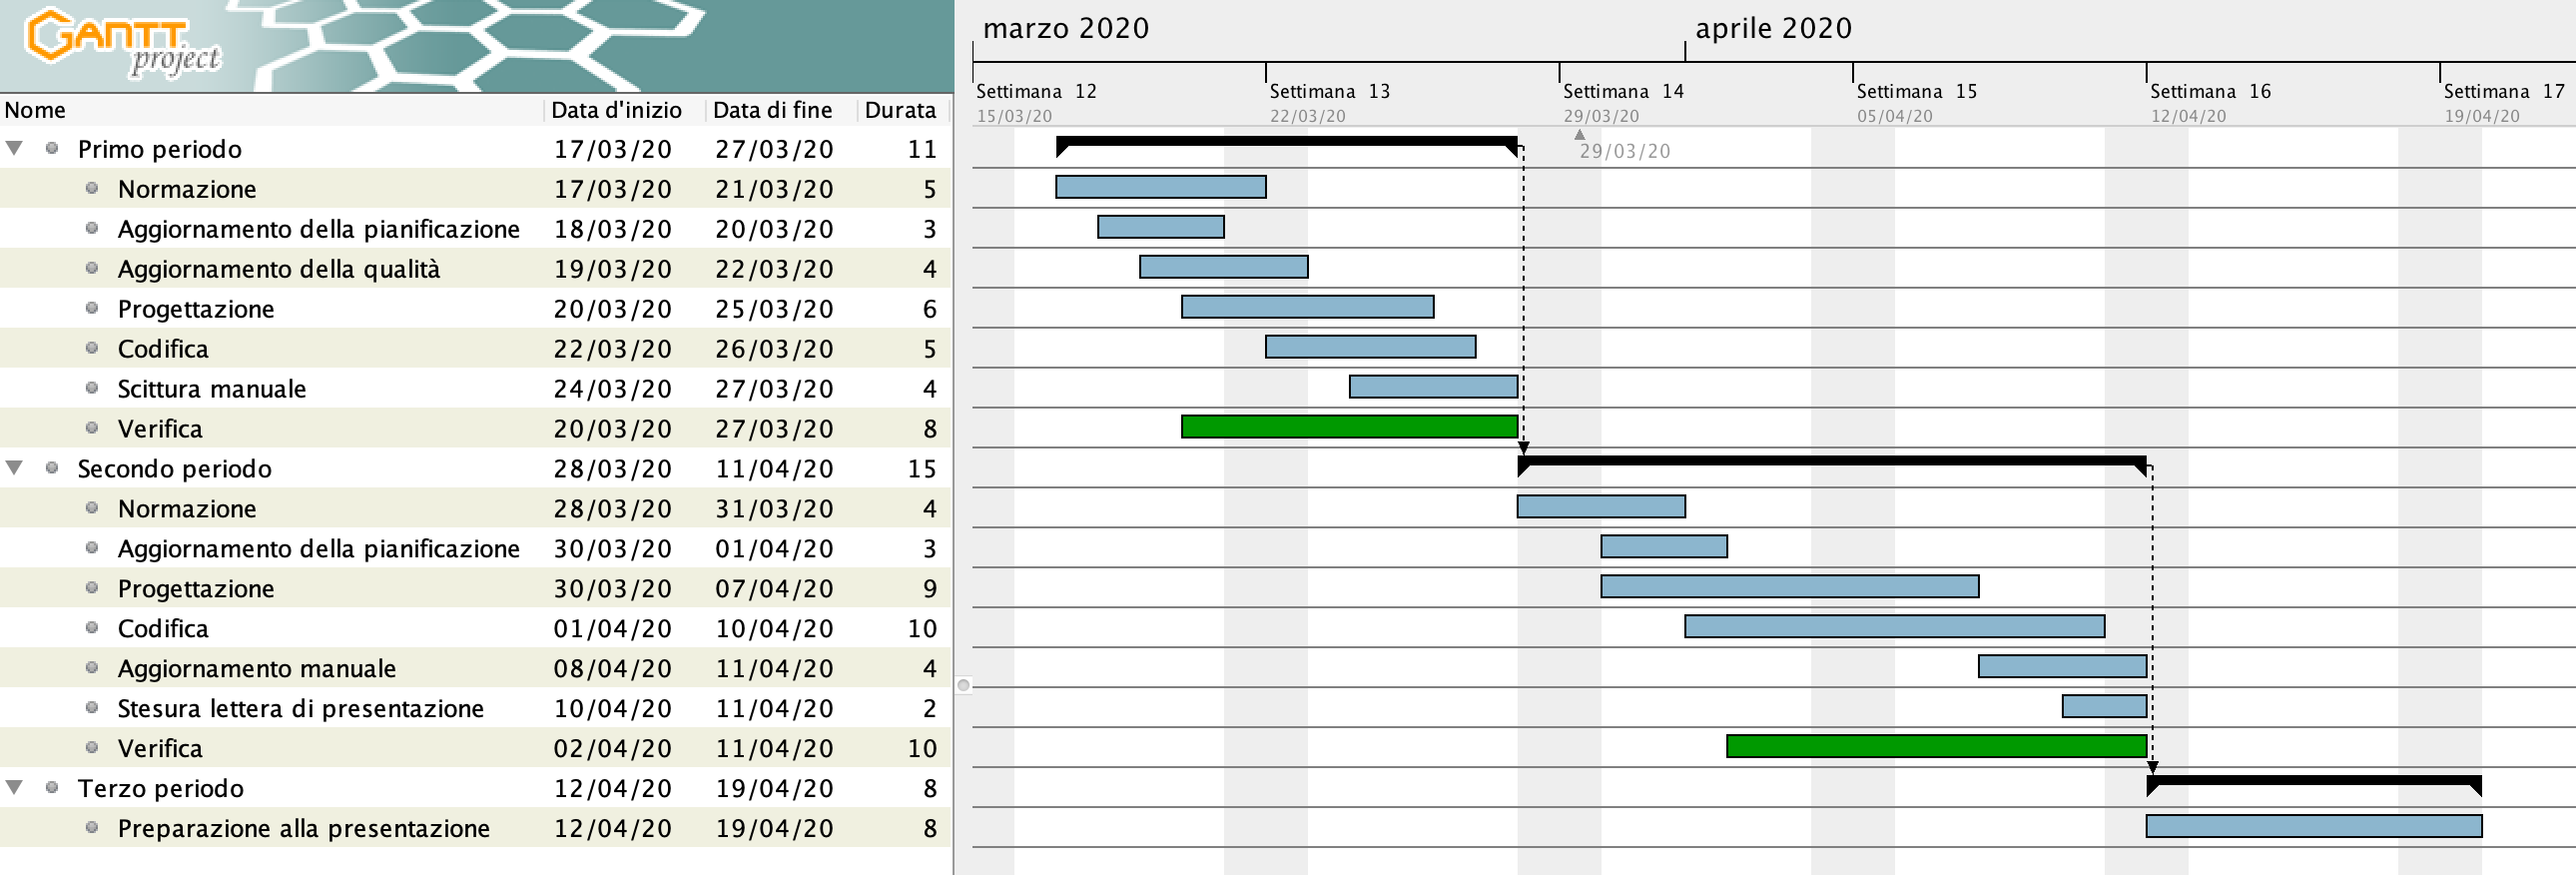
\includegraphics[width=\linewidth]{images/ganttDettaglioCodifica} %TOUPDATE
            \caption{Diagramma di Gantt per l'incremento X}
          \end{figure}		
		\end{landscape}

		% ============================================

		\subsection{Incremento XI}
			
			L'incremento XI prevede la progettazione di dettaglio e codifica delle componenti software. La fase si articola subito prima la revisione di qualifica prevista dal progetto didattico. Si prevede di svolgere quanto segue:
			\begin{itemize}
				\item configurazione aggiuntiva del \glock{gateway} con Kafka;
				\item implementazione completa delle \glock{API}.
			\end{itemize}
			
			\subsubsection{Ruoli attivi}
			
				Durante questa fase è necessaria la presenza dei seguenti ruoli:
				\begin{itemize}
					\item responsabile;
					\item amministratore;
					\item progettista;
					\item programmatore;
					\item verificatore.
				\end{itemize}
			
			\subsubsection{Periodi e attività}
			
				L'incremento viene svolto in un unico periodo di breve durata.
				
				\paragraph{Unico periodo (dal 2020-04-13 al 2020-04-20)}
				
					\begin{itemize}
						\item \textbf{presentazione:} creazione slides per la presentazione del \textit{product baseline};
						\item \textbf{progettazione:} progettazione della comunicazione tra Kafka, \glock{gateway} e dispositivi;
						\item \textbf{codifica:} 
						\begin{itemize}
							\item implementazione conclusiva  tra Kafka, \glock{gateway} e dispositivi; 
							\item implementazione conclusiva delle \glock{API};
						\end{itemize}
						\item \textbf{verifica software:} controllo delle nuove funzionalità tali per cui soddisfino i requisiti predisposti;
						\item \textbf{stesura:} continuazione del \textit{manuale di manutenzione}, integrazione delle funzionalità del \glock{gateway}, delle \glock{API} e dei database;
						\item \textbf{verifica documenti:} verifica delle sezioni aggiunte nel documento modificato.
					\end{itemize} 			

		\begin{landscape}
          \begin{figure}[H]
            \centering
            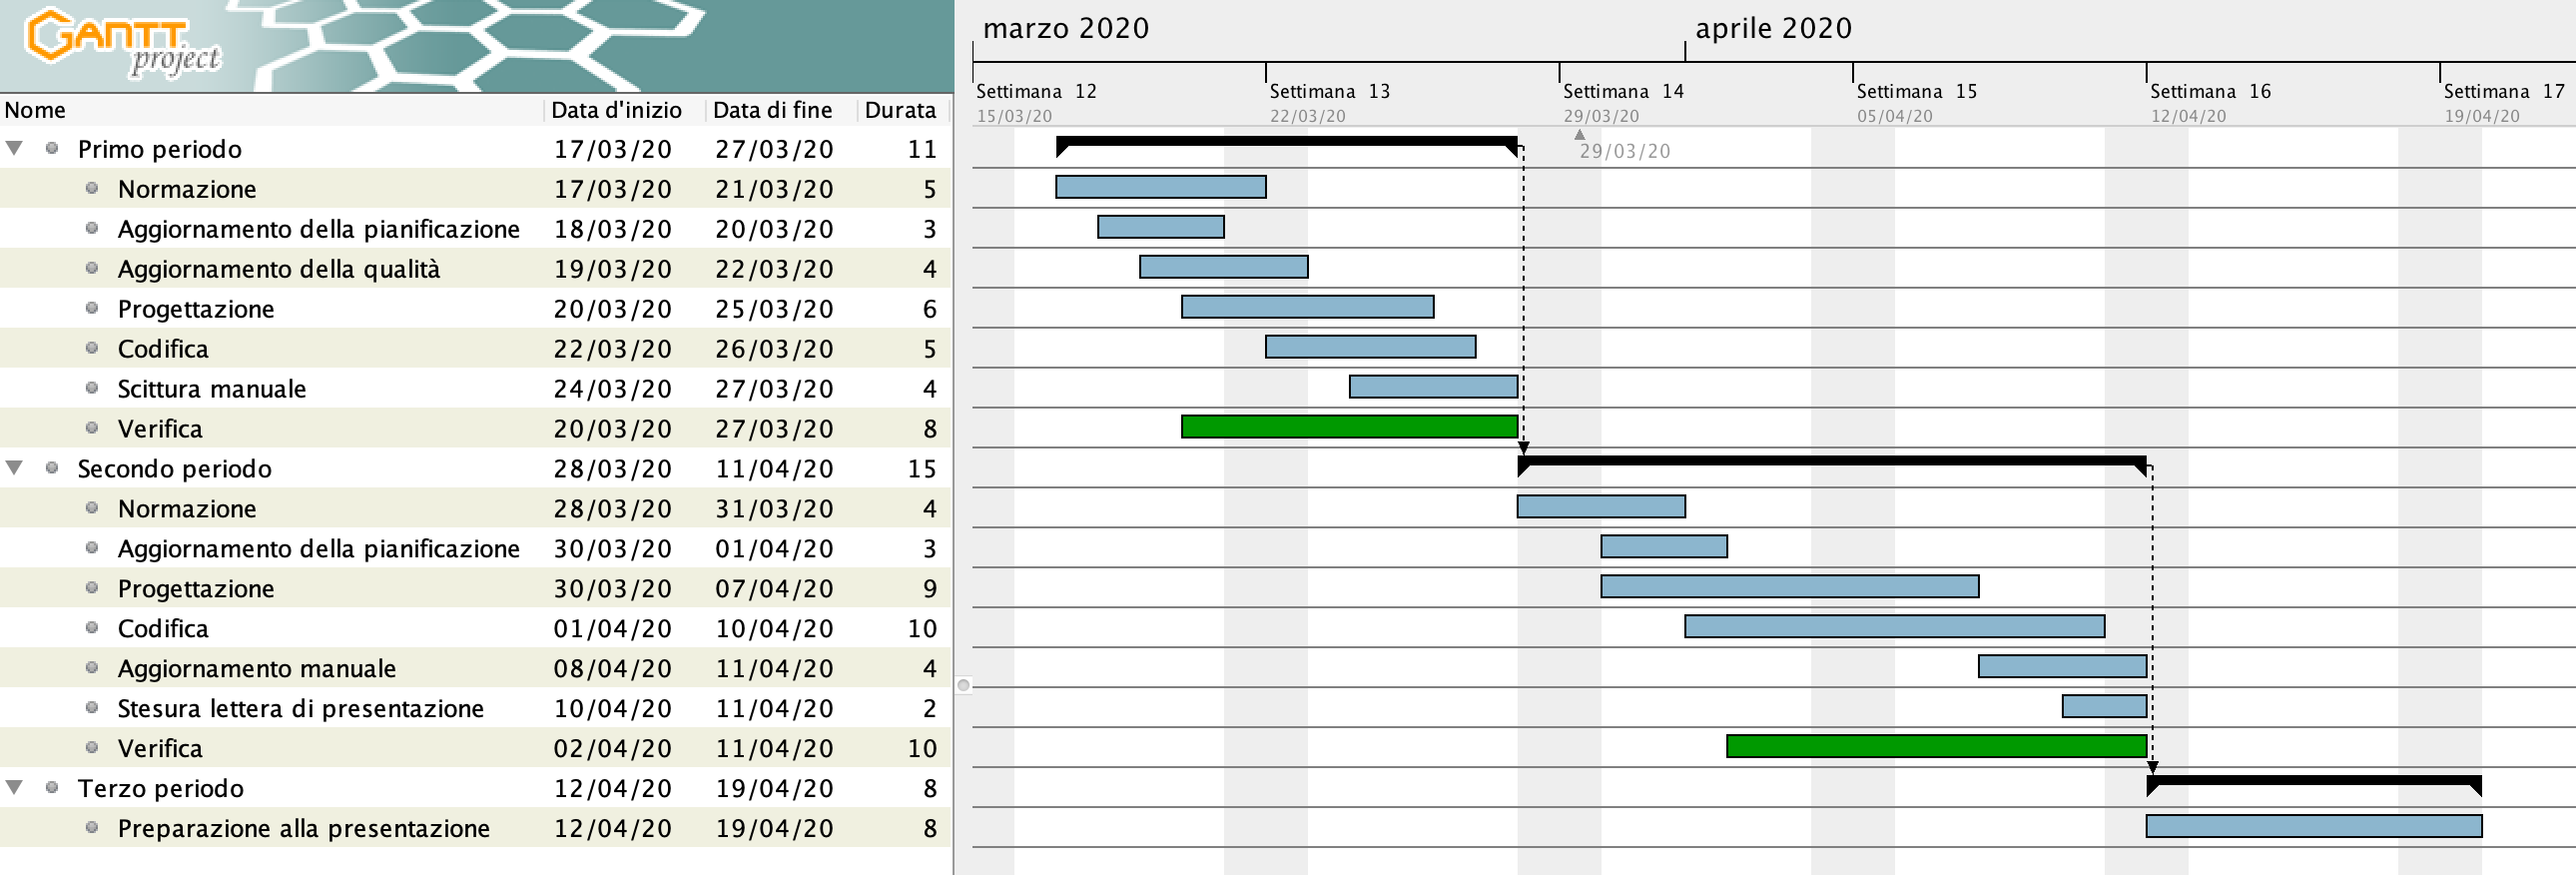
\includegraphics[width=\linewidth]{images/ganttDettaglioCodifica} %TOUPDATE
            \caption{Diagramma di Gantt per l'incremento XI}
          \end{figure}		
		\end{landscape}

		% ============================================

		\subsection{Incremento XII}
			
			L'incremento XII prevede la progettazione di dettaglio e codifica delle componenti software. Si prevede di svolgere quanto segue:
			\begin{itemize}
				\item implementazione invio input con il \glock{bot Telegram};
				\item implementazione amministrazione web app.
			\end{itemize}
			
			\subsubsection{Ruoli attivi}
			
				Durante questa fase è necessaria la presenza dei seguenti ruoli:
				\begin{itemize}
					\item responsabile;
					\item amministratore;
					\item progettista;
					\item programmatore;
					\item verificatore.
				\end{itemize}
			
			\subsubsection{Periodi e attività}
			
				L'incremento viene svolto in un unico periodo di breve durata.
				
				\paragraph{Unico periodo (dal 2020-04-21 al 2020-04-30)}
				
					\begin{itemize}
						\item \textbf{progettazione:} 
						\begin{itemize}
							\item progettazione dell'invio input a un dispositivo con il \glock{bot Telegram};
							\item progettazione dell'amministrazione nella web app;
						\end{itemize}
						\item \textbf{codifica:} 
						\begin{itemize}
							\item implementazione conclusiva del \glock{bot Telegram} con le funzionalità di invio input a un dispositivo; 
							\item implementazione della parte amministrativa della web app;
							\item implementazione di eventuali ritocchi grafici necessari;
						\end{itemize}
						\item \textbf{verifica software:} controllo delle nuove funzionalità tali per cui soddisfino i requisiti predisposti;
						\item \textbf{stesura:} 
						\begin{itemize}
							\item \textit{manuale di manutenzione:} integrazione delle funzionalità della parte amministrativa e del \glock{bot Telegram};
							\item \textit{manuale utente:} descrizione delle funzionalità per un amministratore;
						\end{itemize}
						\item \textbf{verifica documenti:} verifica delle sezioni aggiunte nel documento modificato.
					\end{itemize} 			

		\begin{landscape}
          \begin{figure}[H]
            \centering
            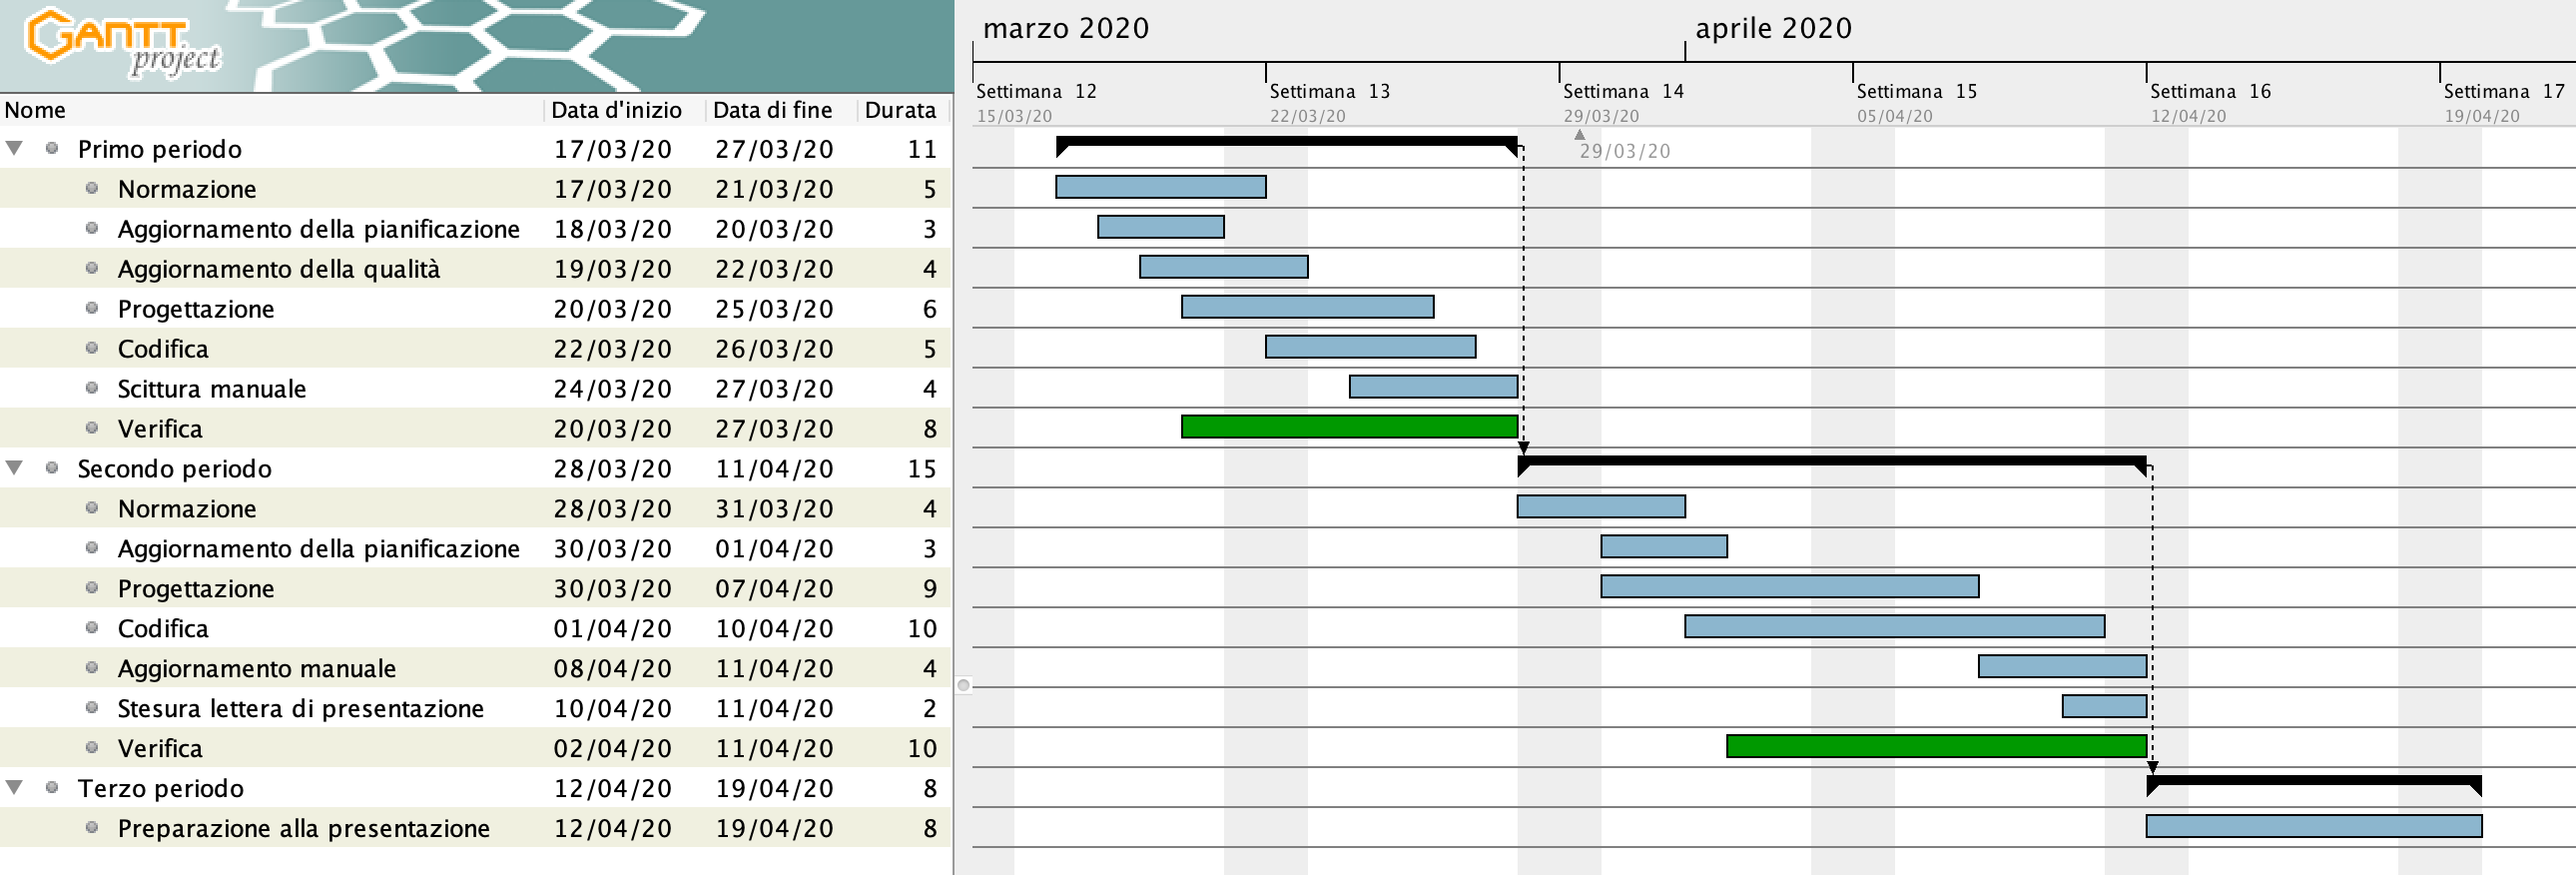
\includegraphics[width=\linewidth]{images/ganttDettaglioCodifica} %TOUPDATE
            \caption{Diagramma di Gantt per l'incremento XII}
          \end{figure}		
		\end{landscape}

		% ============================================

		\subsection{Validazione e collaudo}	
		
			L'attività di validazione e collaudo ha inizio il giorno 2020-04-21, successivamente alla revisione di qualifica, ed è suddivisa in due periodi, con termine fissato per il giorno 2020-05-17, che precede la revisione di accettazione del 2020-05-18.
			
			\subsubsection{Ruoli attivi}
			
			Durante questa attività è necessaria la presenza dei seguenti ruoli:
			\begin{itemize}
				\item responsabile;
				\item amministratore;
				\item progettista;
				\item programmatore;
				\item verificatore.
			\end{itemize}
			
			\subsubsection{Periodi}
			
				L'attività di validazione e collaudo è stata suddivisa nei seguenti periodi:
		
				\paragraph{Primo periodo (dal 2020-05-01 al 2020-05-11)}
			
					\begin{itemize}
						\item \textbf{normazione:} revisione ed eventuale aggiornamento delle norme;
						\item \textbf{aggiornamento della pianificazione};
						\item \textbf{aggiornamento della qualità};
						% \item \textbf{completamento progettazione};
						\item \textbf{verifica:} controllo della qualità di tutti i prodotti sviluppati durante il periodo attuale.
					\end{itemize} 	
				
				\paragraph{Secondo periodo (dal 2020-05-12 al 2020-05-17)}
				
					\begin{itemize}
						\item \textbf{codifica:} rilascio ultima versione;
						\item \textbf{completamento manuale};
						\item \textbf{verifica:} controllo della qualità di tutti i prodotti sviluppati durante il periodo attuale, in particolare sono eseguiti i test per la verifica del software.
					\end{itemize}

			
		\begin{landscape}

          \begin{figure}[H]
            \centering
            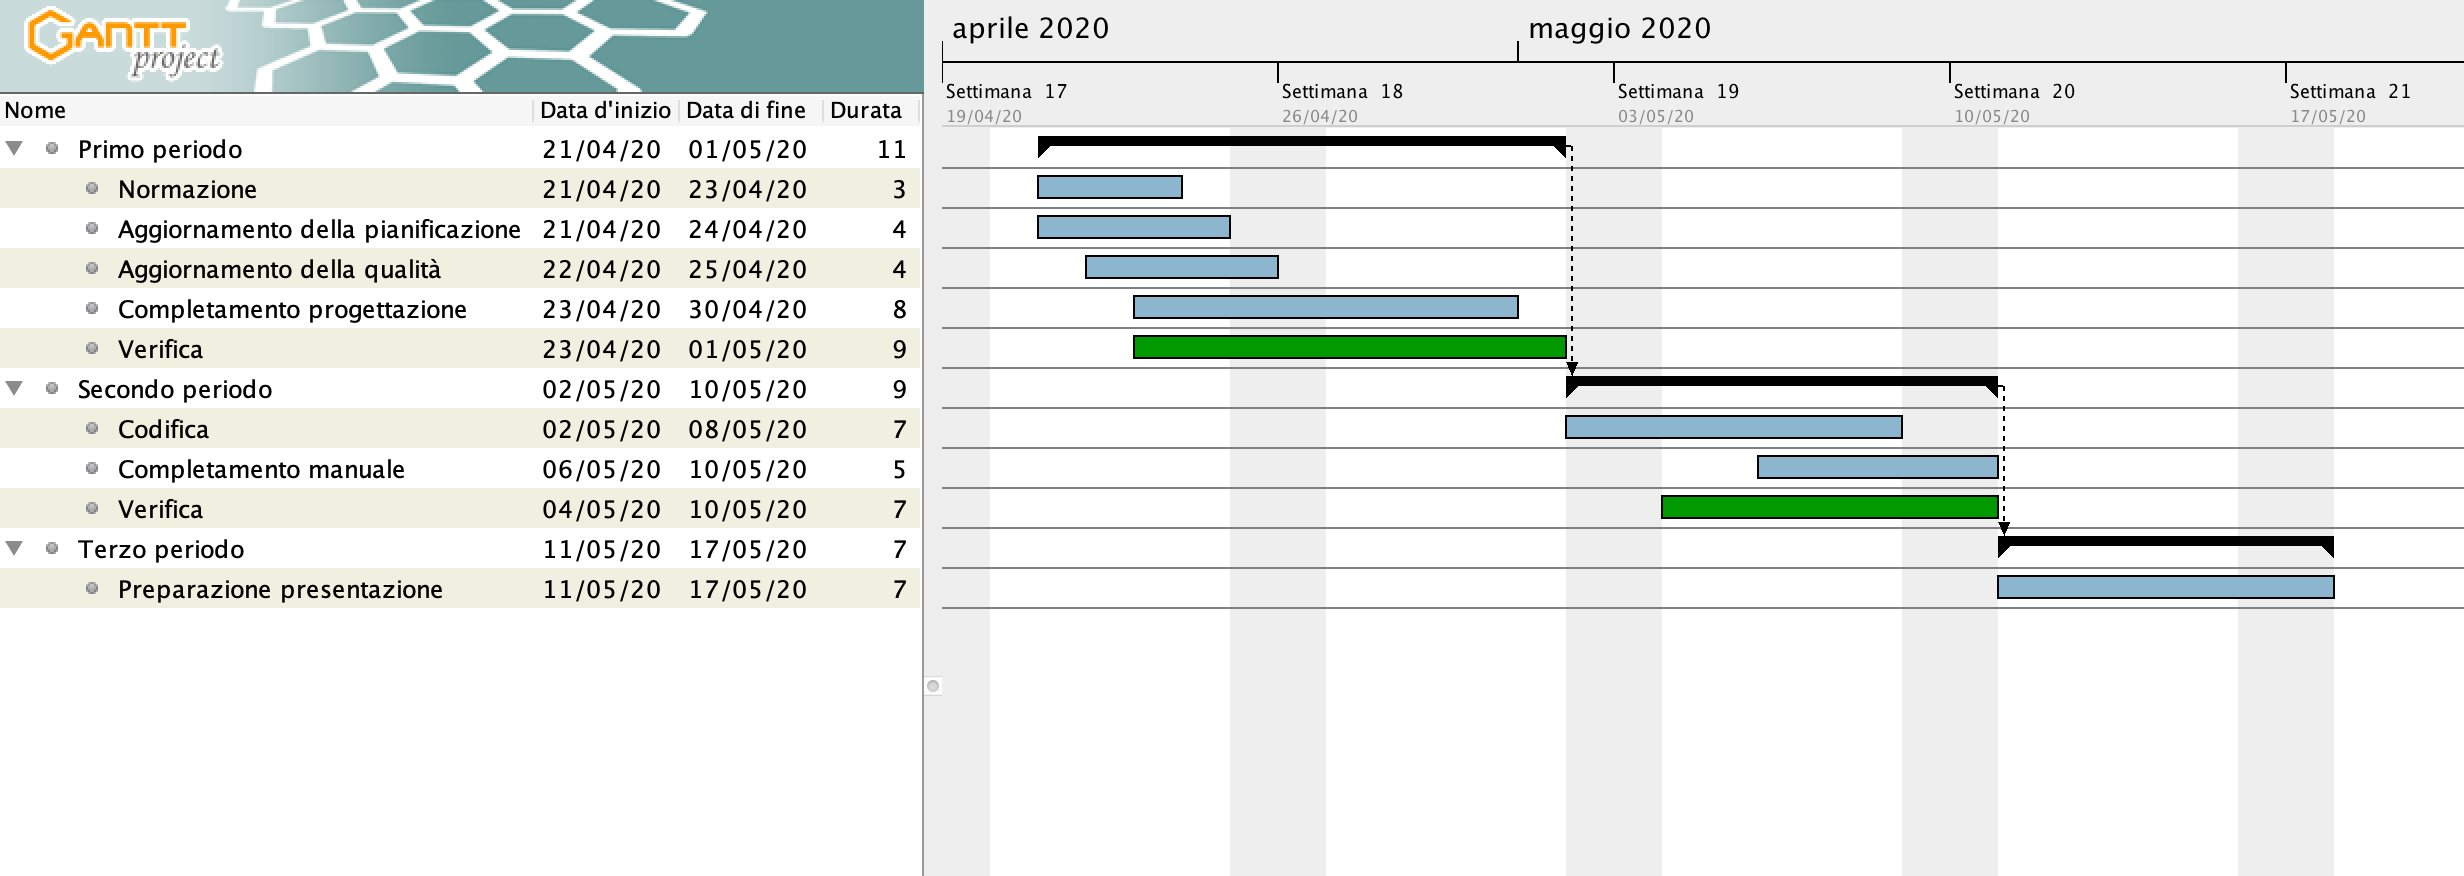
\includegraphics[width=\linewidth]{images/ganttValidazioneColl}
            \caption{Diagramma di Gantt dell'attività di validazione e collaudo}
          \end{figure}

		\end{landscape}
